\section{What I Have Done}
\begin{frame}{General Remarks}
    \begin{itemize}
        \item \texttt{dnn\_reco} running on the IceCube servers and cluster @Wisconsin
        \item I modified a few python scripts of the original software to add minor functionalities\footnote{Can be found \href{https://github.com/The-Ludwig/dnn_reco}{here: github.com/The-Ludwig/dnn\_reco} }
        \item Submit-scripts to work with the cluster GPUs were created
        \item Noted where \texttt{dnn\_reco}'s documentation\footnote{Documentation can be found \href{https://user-web.icecube.wisc.edu/~mhuennefeld/docs/dnn_reco/html/pages/about.html}{here}} is out-of-date
    \end{itemize}

    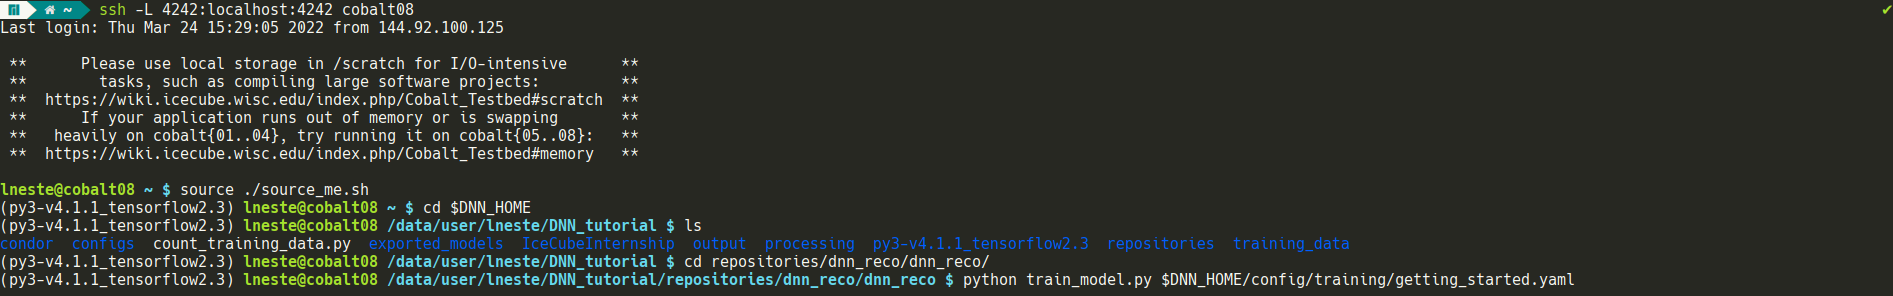
\includegraphics[width=\textwidth]{media/console.png}
\end{frame}
\begin{frame}{A First Model @13000 Training Iterations}
    \begin{columns}
        \begin{column}{.35\textwidth}
            \begin{tabular}{>{\small\bf}r l}
                \toprule
                Features                  & 9                \\
                Training Dataset          & L2 11883         \\
                Batch Size                & 32               \\
                UDC conv. layers          & 4                \\
                LDC conv. layers          & 8                \\
                Hex. conv. layers         & 8                \\
                Dense layers              & 1\times50        \\
                $\rightarrow$ Free Params & 24532            \\
                \midrule
                Test Dataset              & L2 11069         \\
                Loss function             & GL               \\
                Optimizer                 & ADAM             \\
                Learning Rate             & $10^{-3}$        \\
                Input Dropout Rate        & \SI{5}{\percent} \\
                \bottomrule
            \end{tabular}
        \end{column}
        \begin{column}{.65\textwidth}
            \begin{figure}
                \centering
                \only<1>{
                    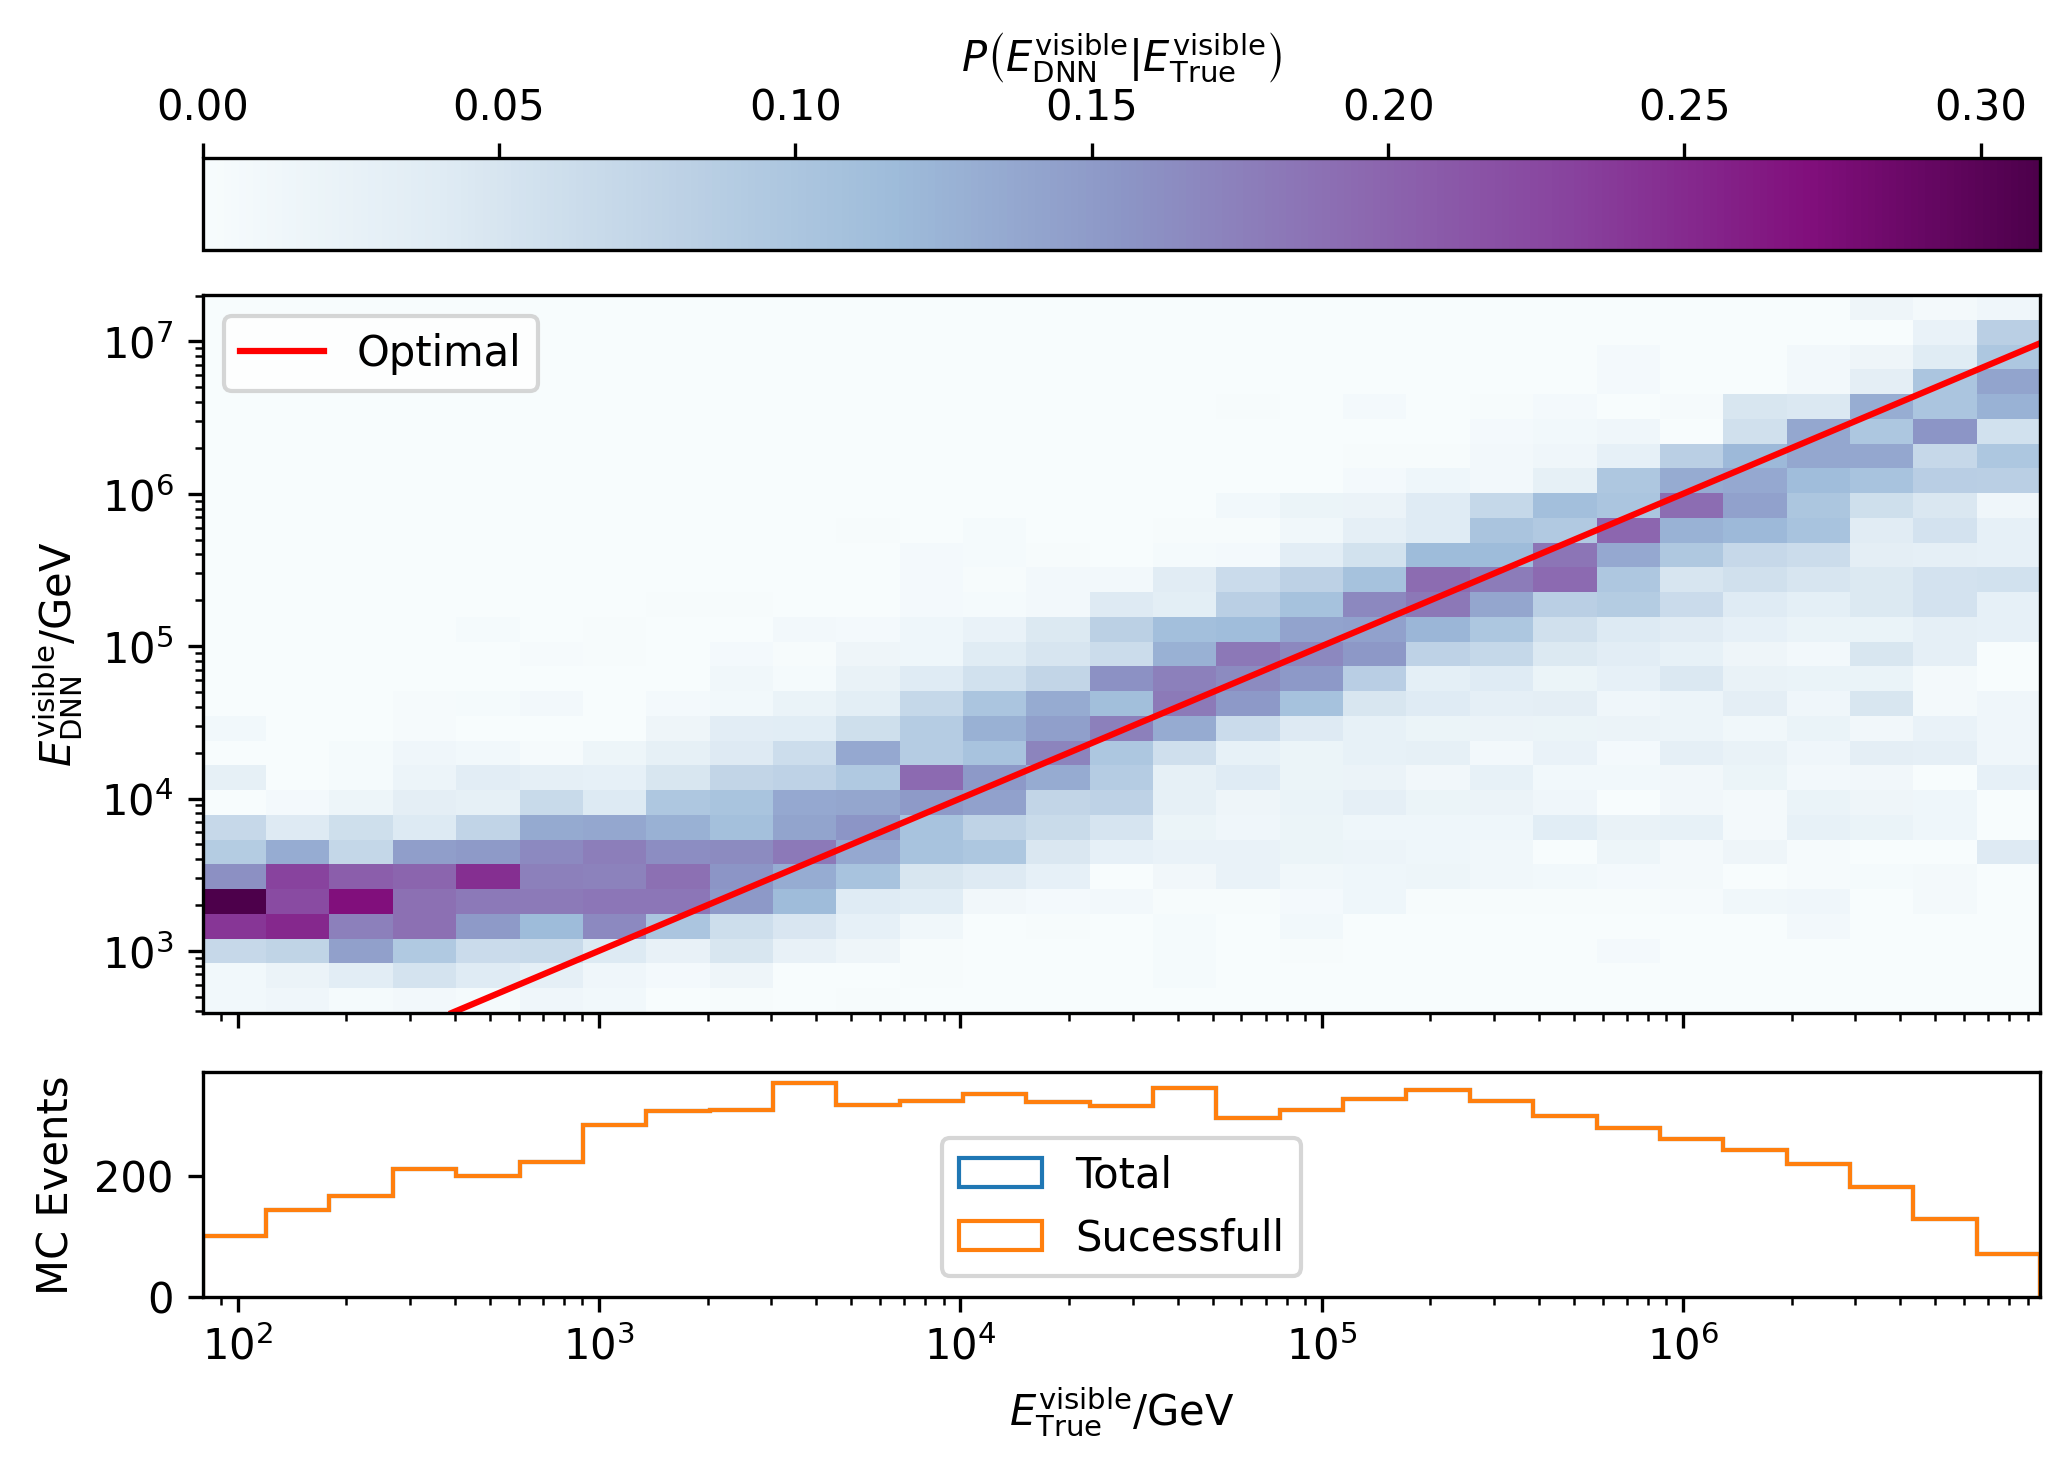
\includegraphics[width=.95\textwidth]{media/DNN_CORR.png}
                    \caption*{\small Normalized correlation plot of visible energy}
                }
                \only<2>{
                    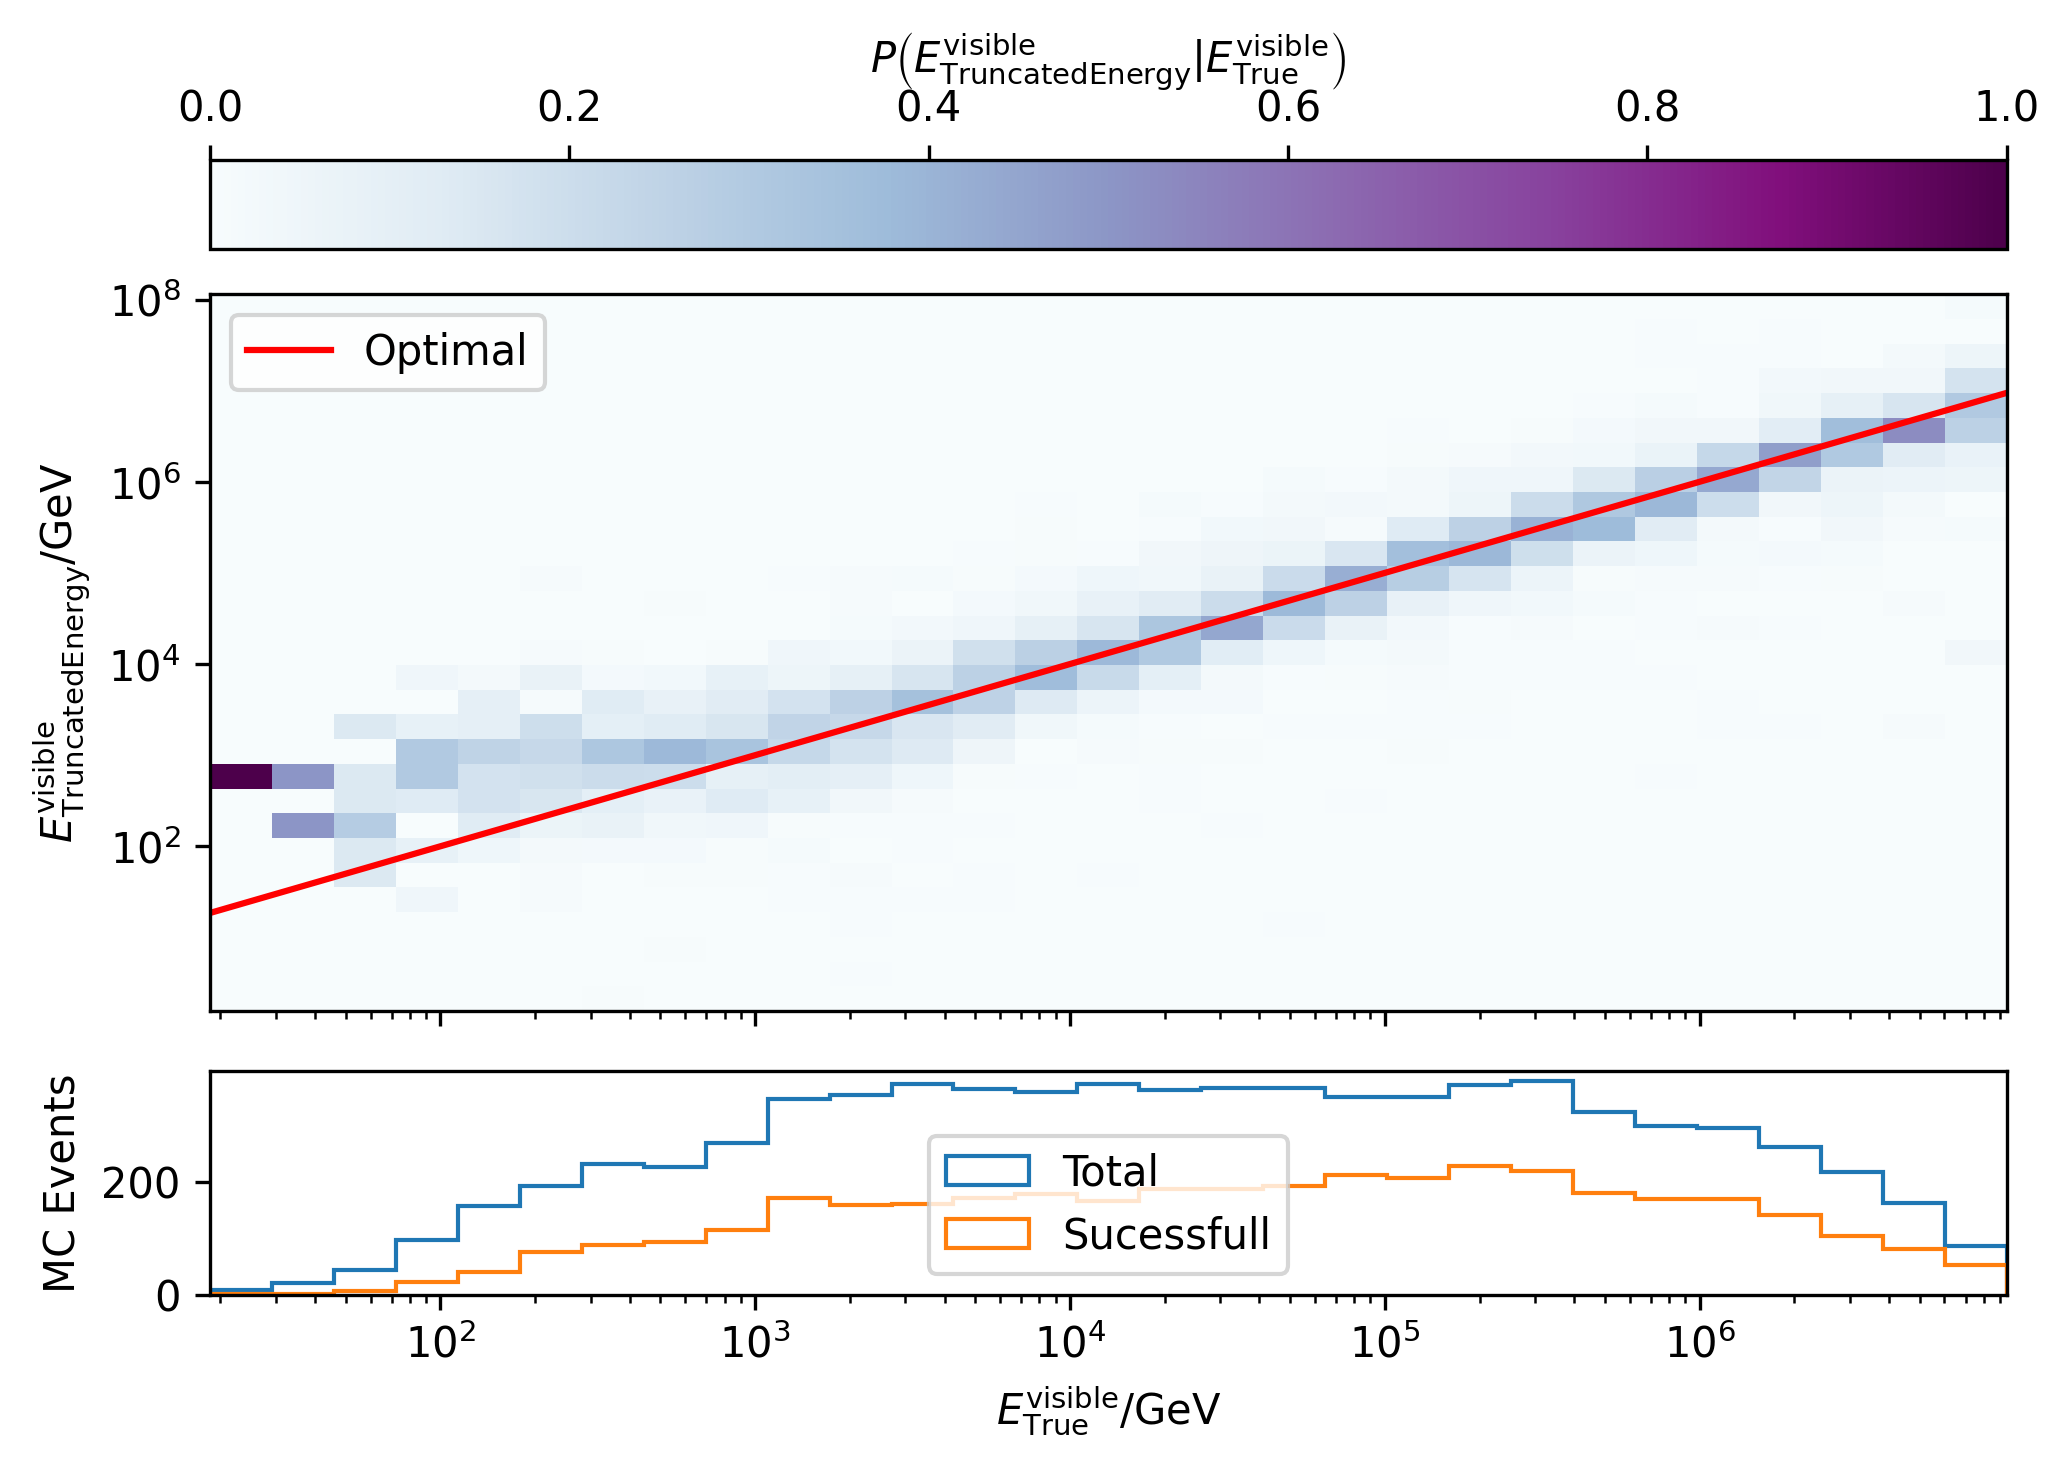
\includegraphics[width=.95\textwidth]{media/TRUN_CORR.png}
                    \caption*{\small Normalized correlation plot of visible energy (classical method)}
                }
            \end{figure}
        \end{column}
    \end{columns}
\end{frame}
\begin{frame}{A First Model for Directional Reconstruction}
    \begin{columns}
        \begin{column}{.35\textwidth}
            \begin{tabular}{>{\small\bf}r l}
                \toprule
                Features                  & 9         \\
                Training Dataset          & L2 11883  \\
                Batch Size                & 32        \\
                UDC conv. layers          & 4         \\
                LDC conv. layers          & 8         \\
                Hex. conv. layers         & 8         \\
                Dense layers              & 1\times50 \\
                $\rightarrow$ Free Params & 24532     \\
                \bottomrule
            \end{tabular}
        \end{column}
        \begin{column}{.65\textwidth}
            \begin{figure}
                \centering
                \only<1>{
                    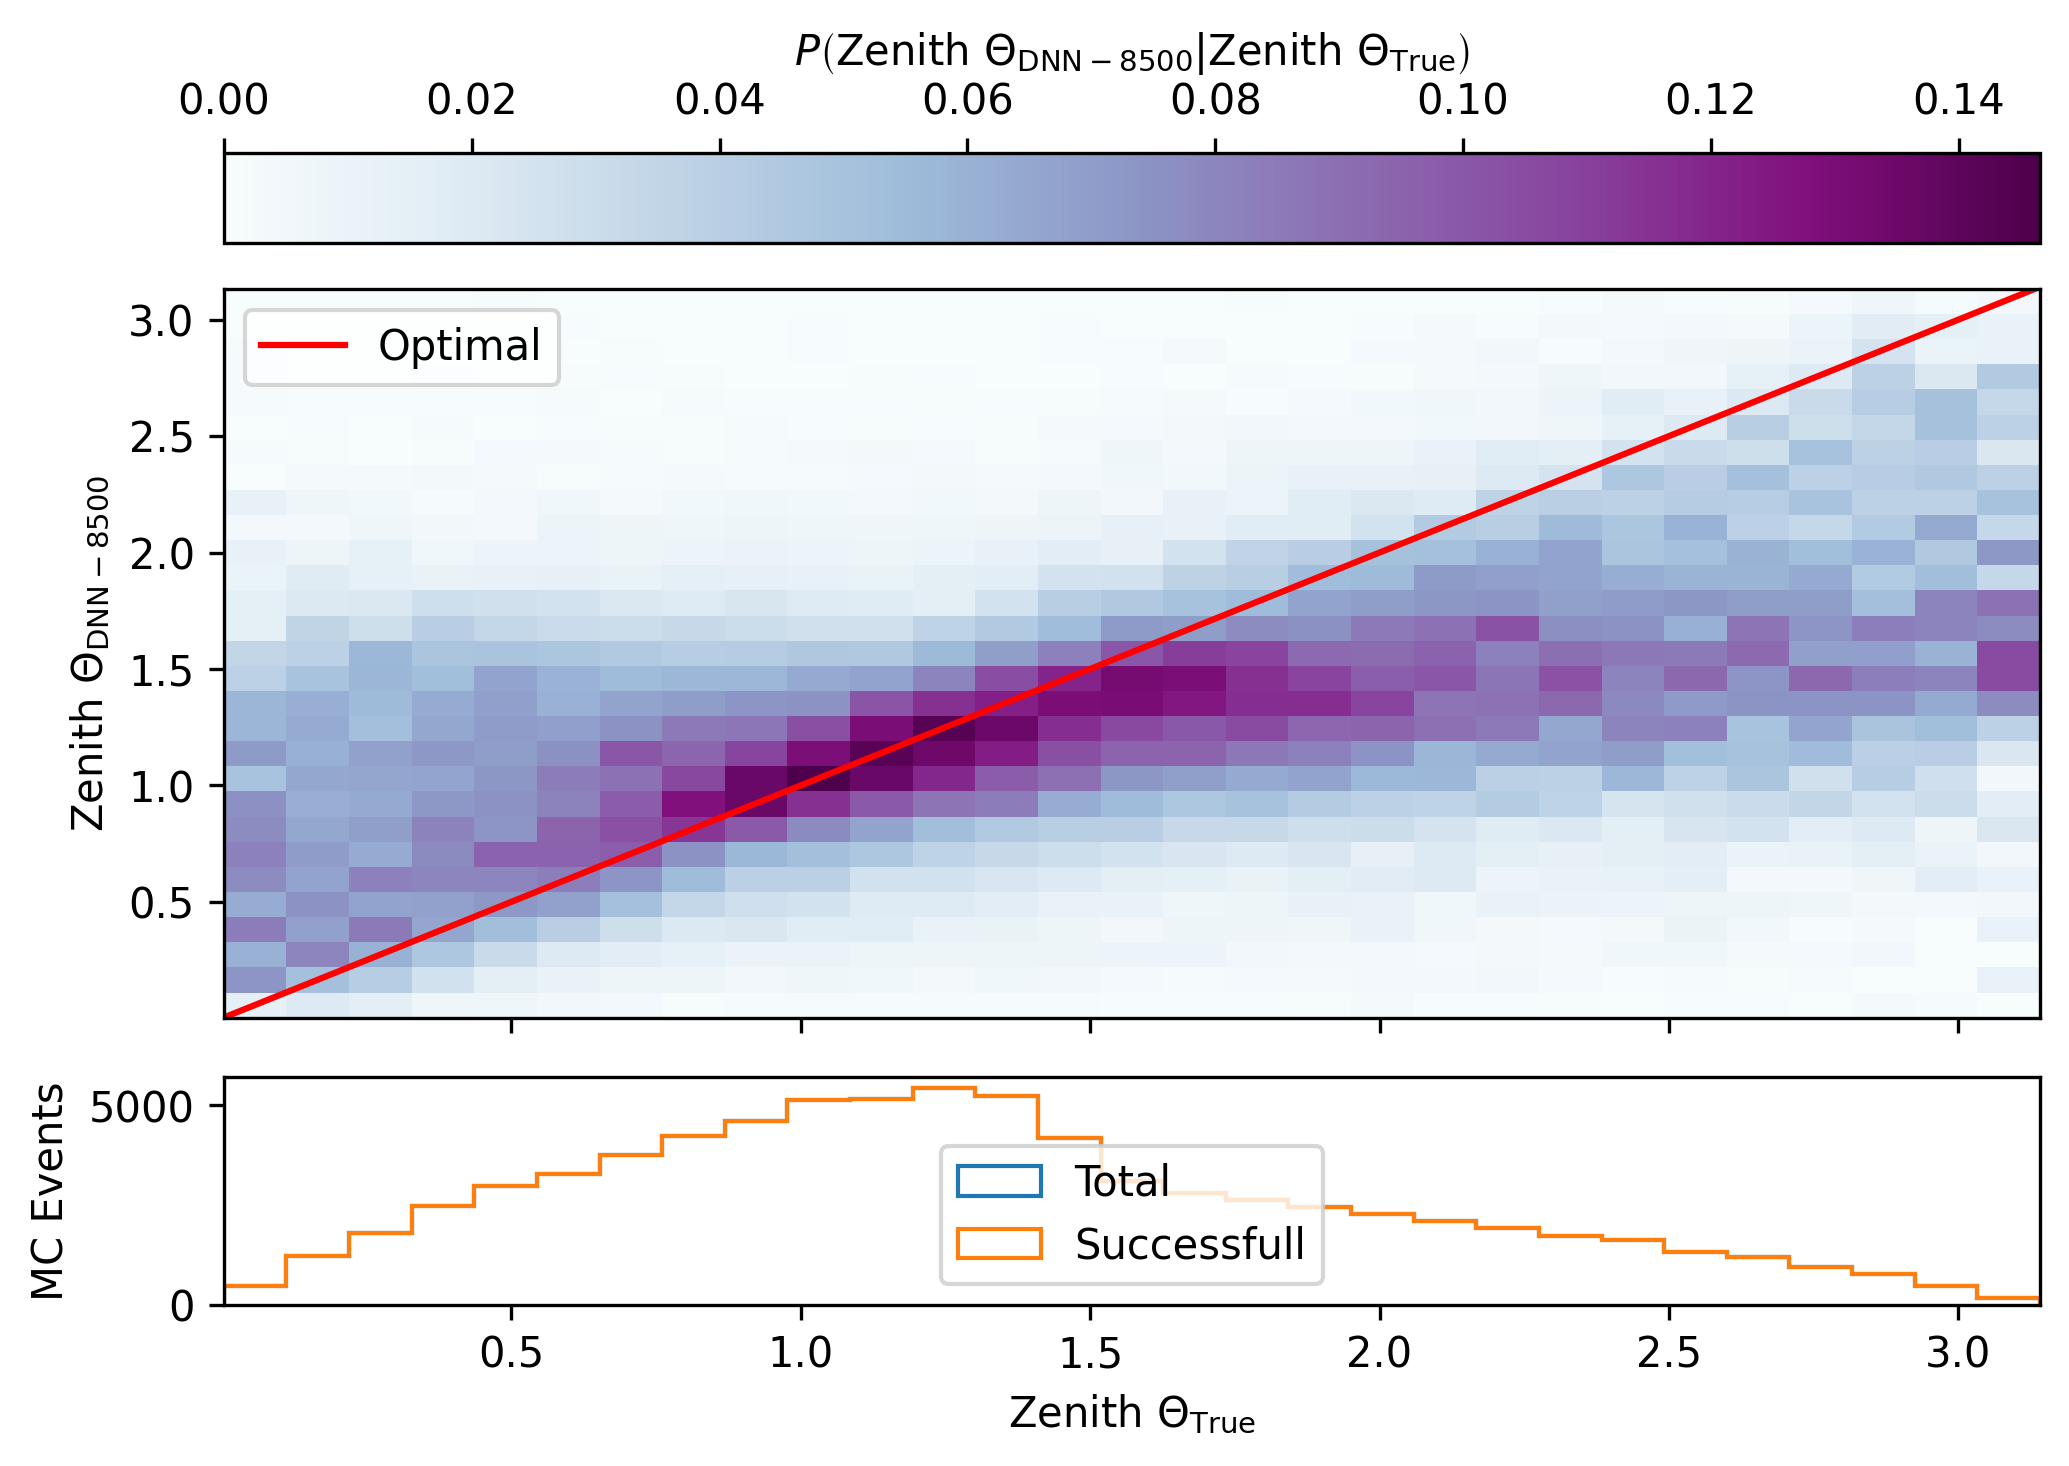
\includegraphics[width=.95\textwidth]{media/zenith_8500.png}
                    \caption*{\small Normalized zenith correlation @8500 training steps}
                }
                \only<2>{
                    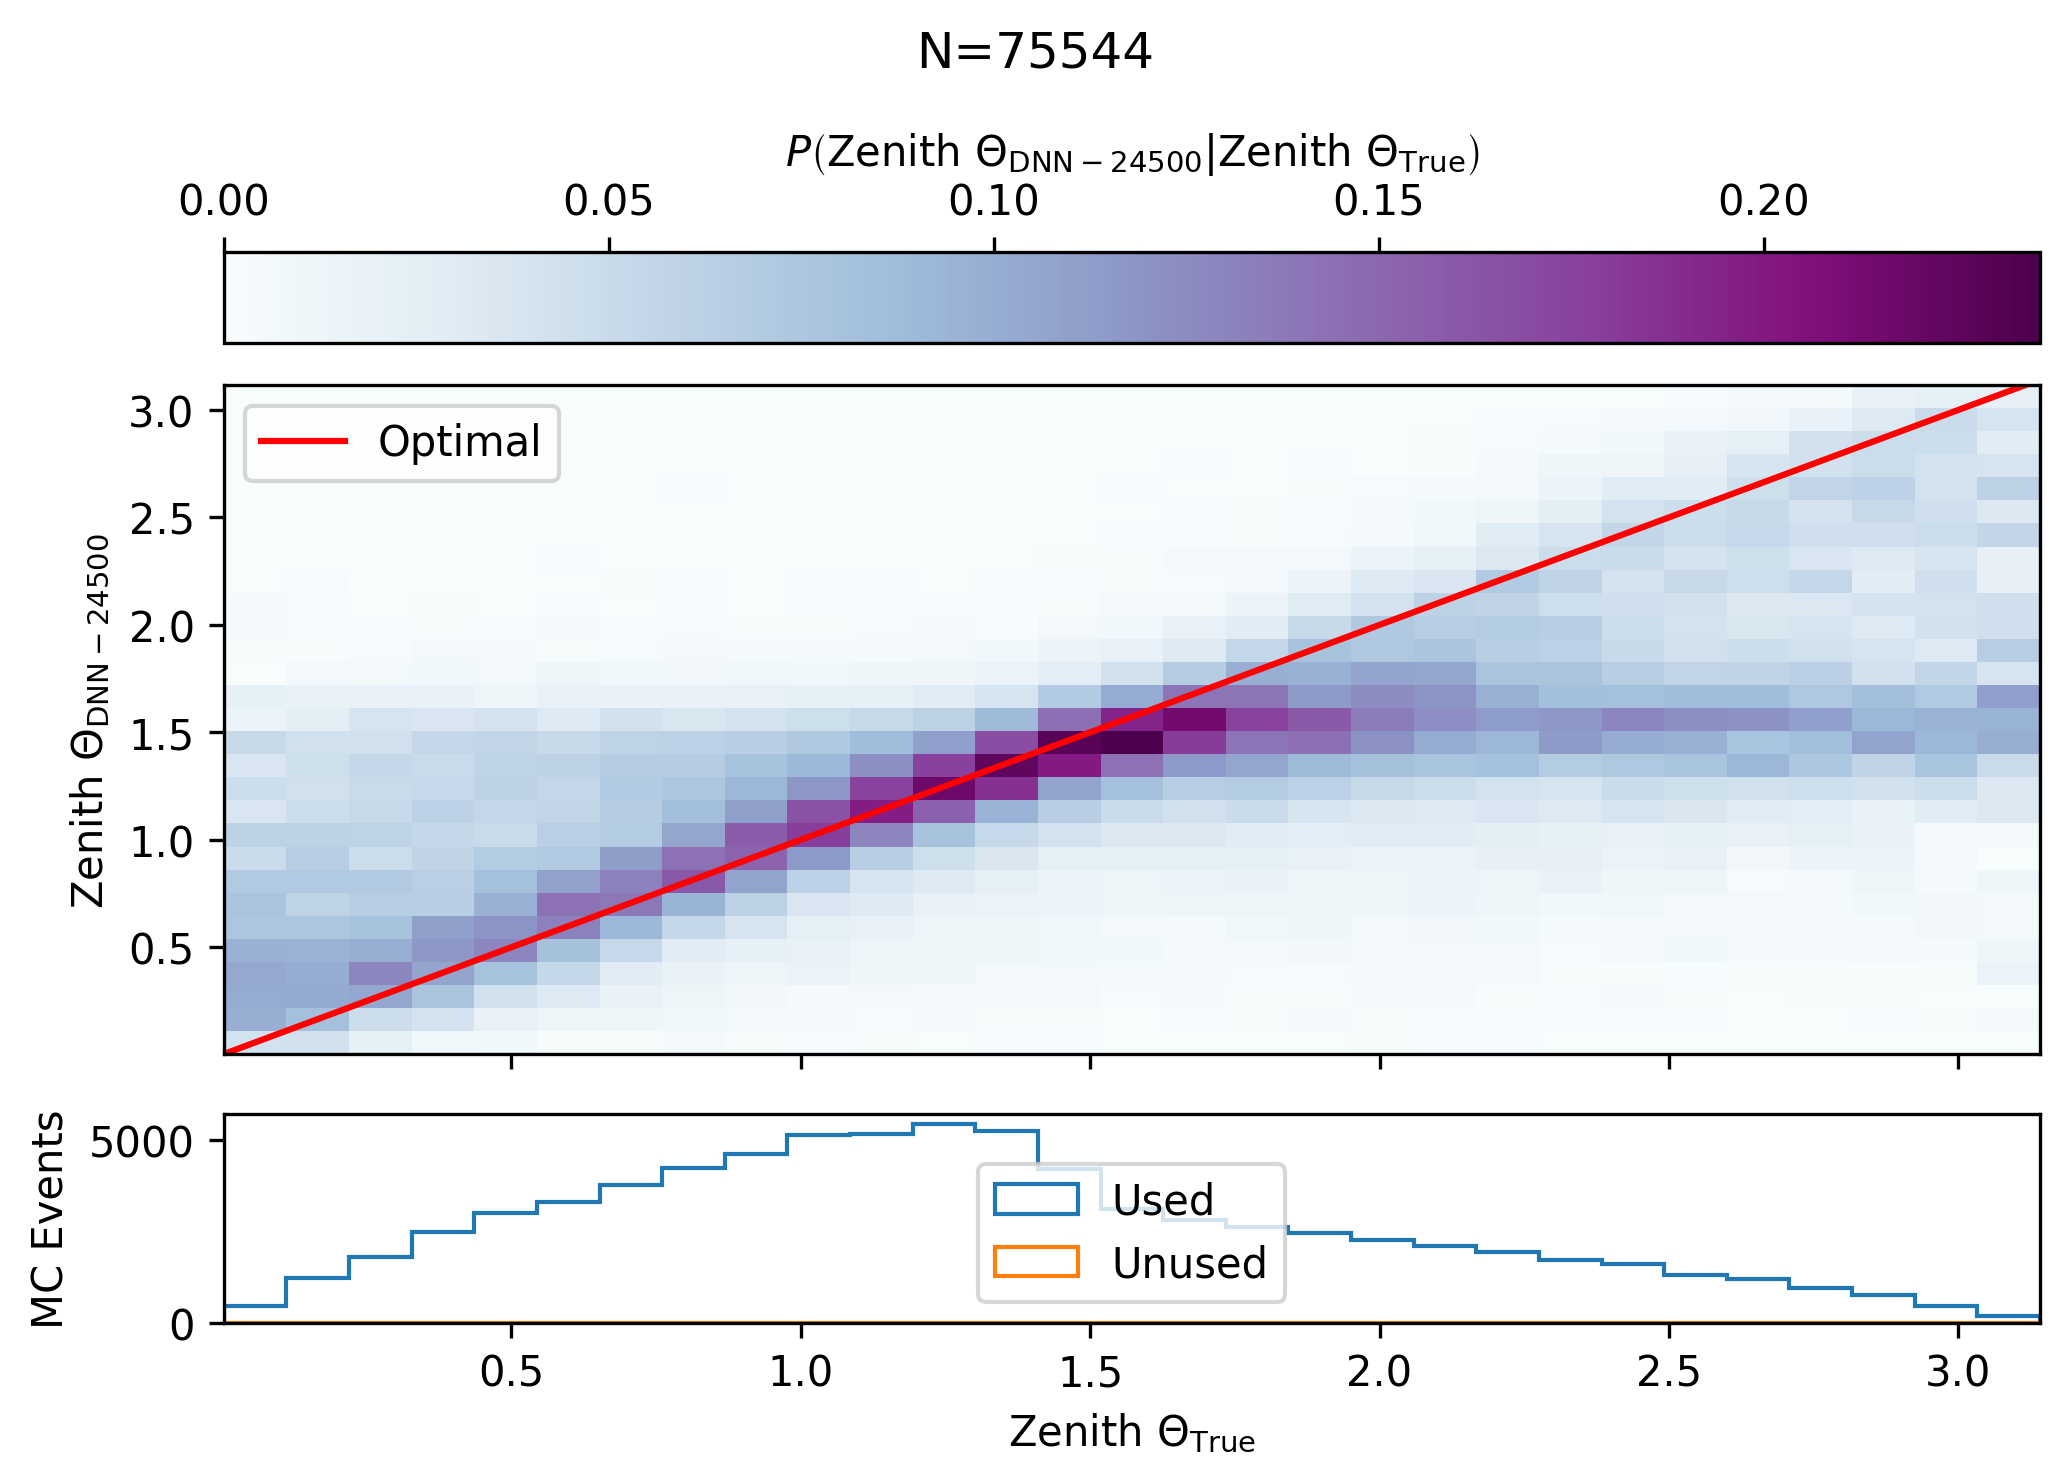
\includegraphics[width=.95\textwidth]{media/zenith_24500.png}
                    \caption*{\small Normalized zenith correlation @24500 training steps}
                }
                \only<3>{
                    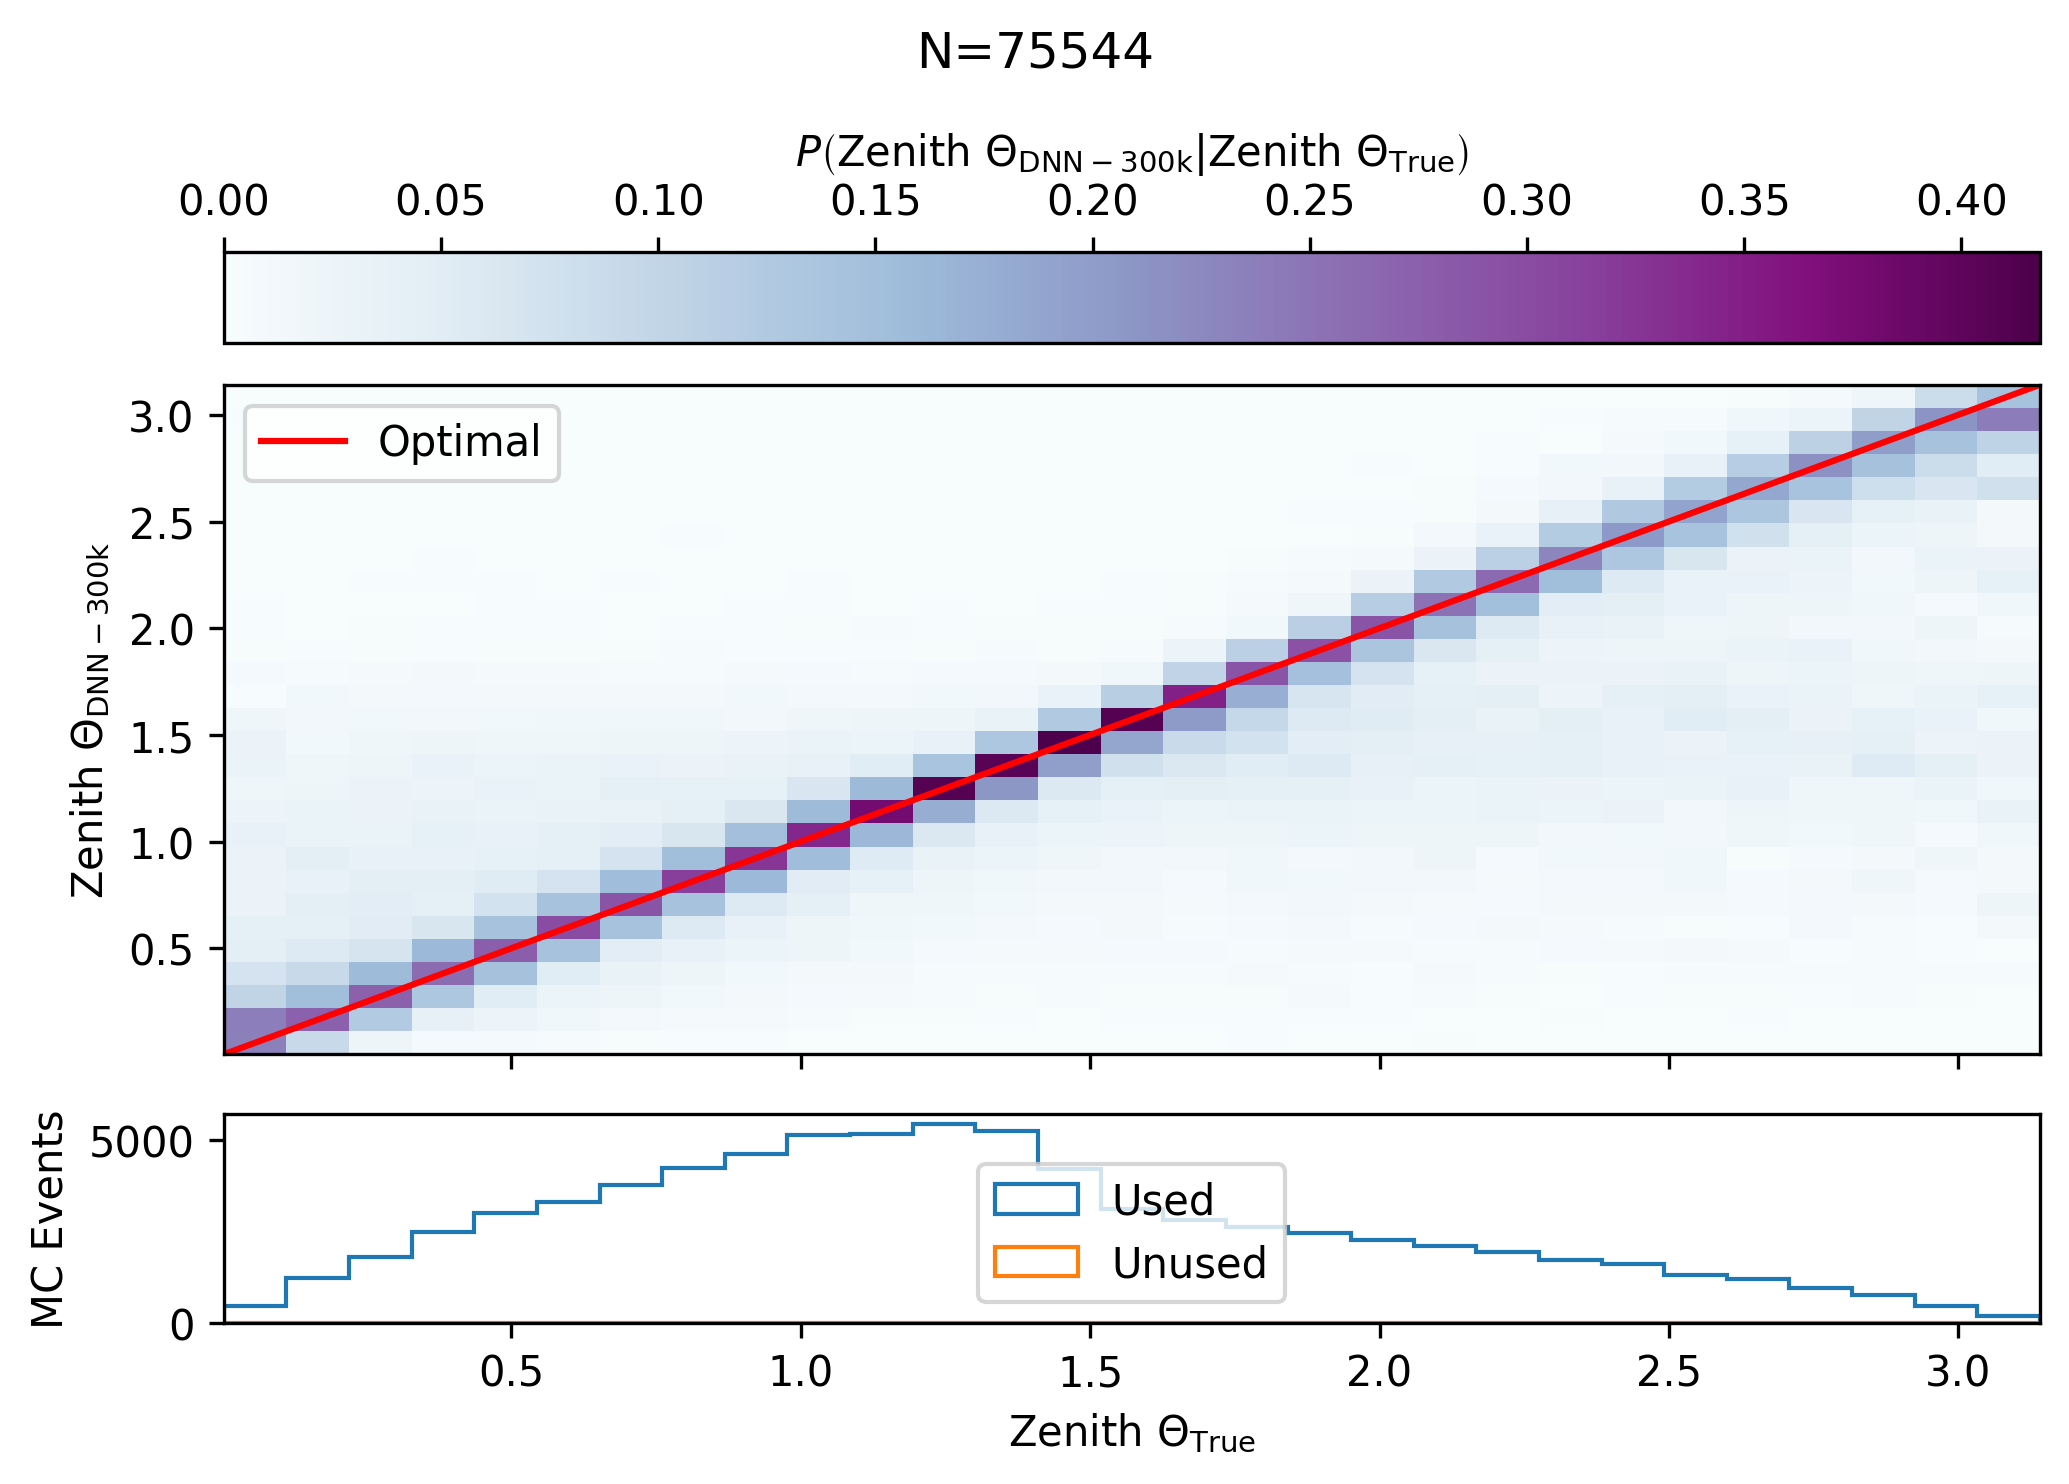
\includegraphics[width=.95\textwidth]{media/zenith_300k.png}
                    \caption*{\small Normalized zenith correlation @300k training steps}
                }
                \only<4>{
                    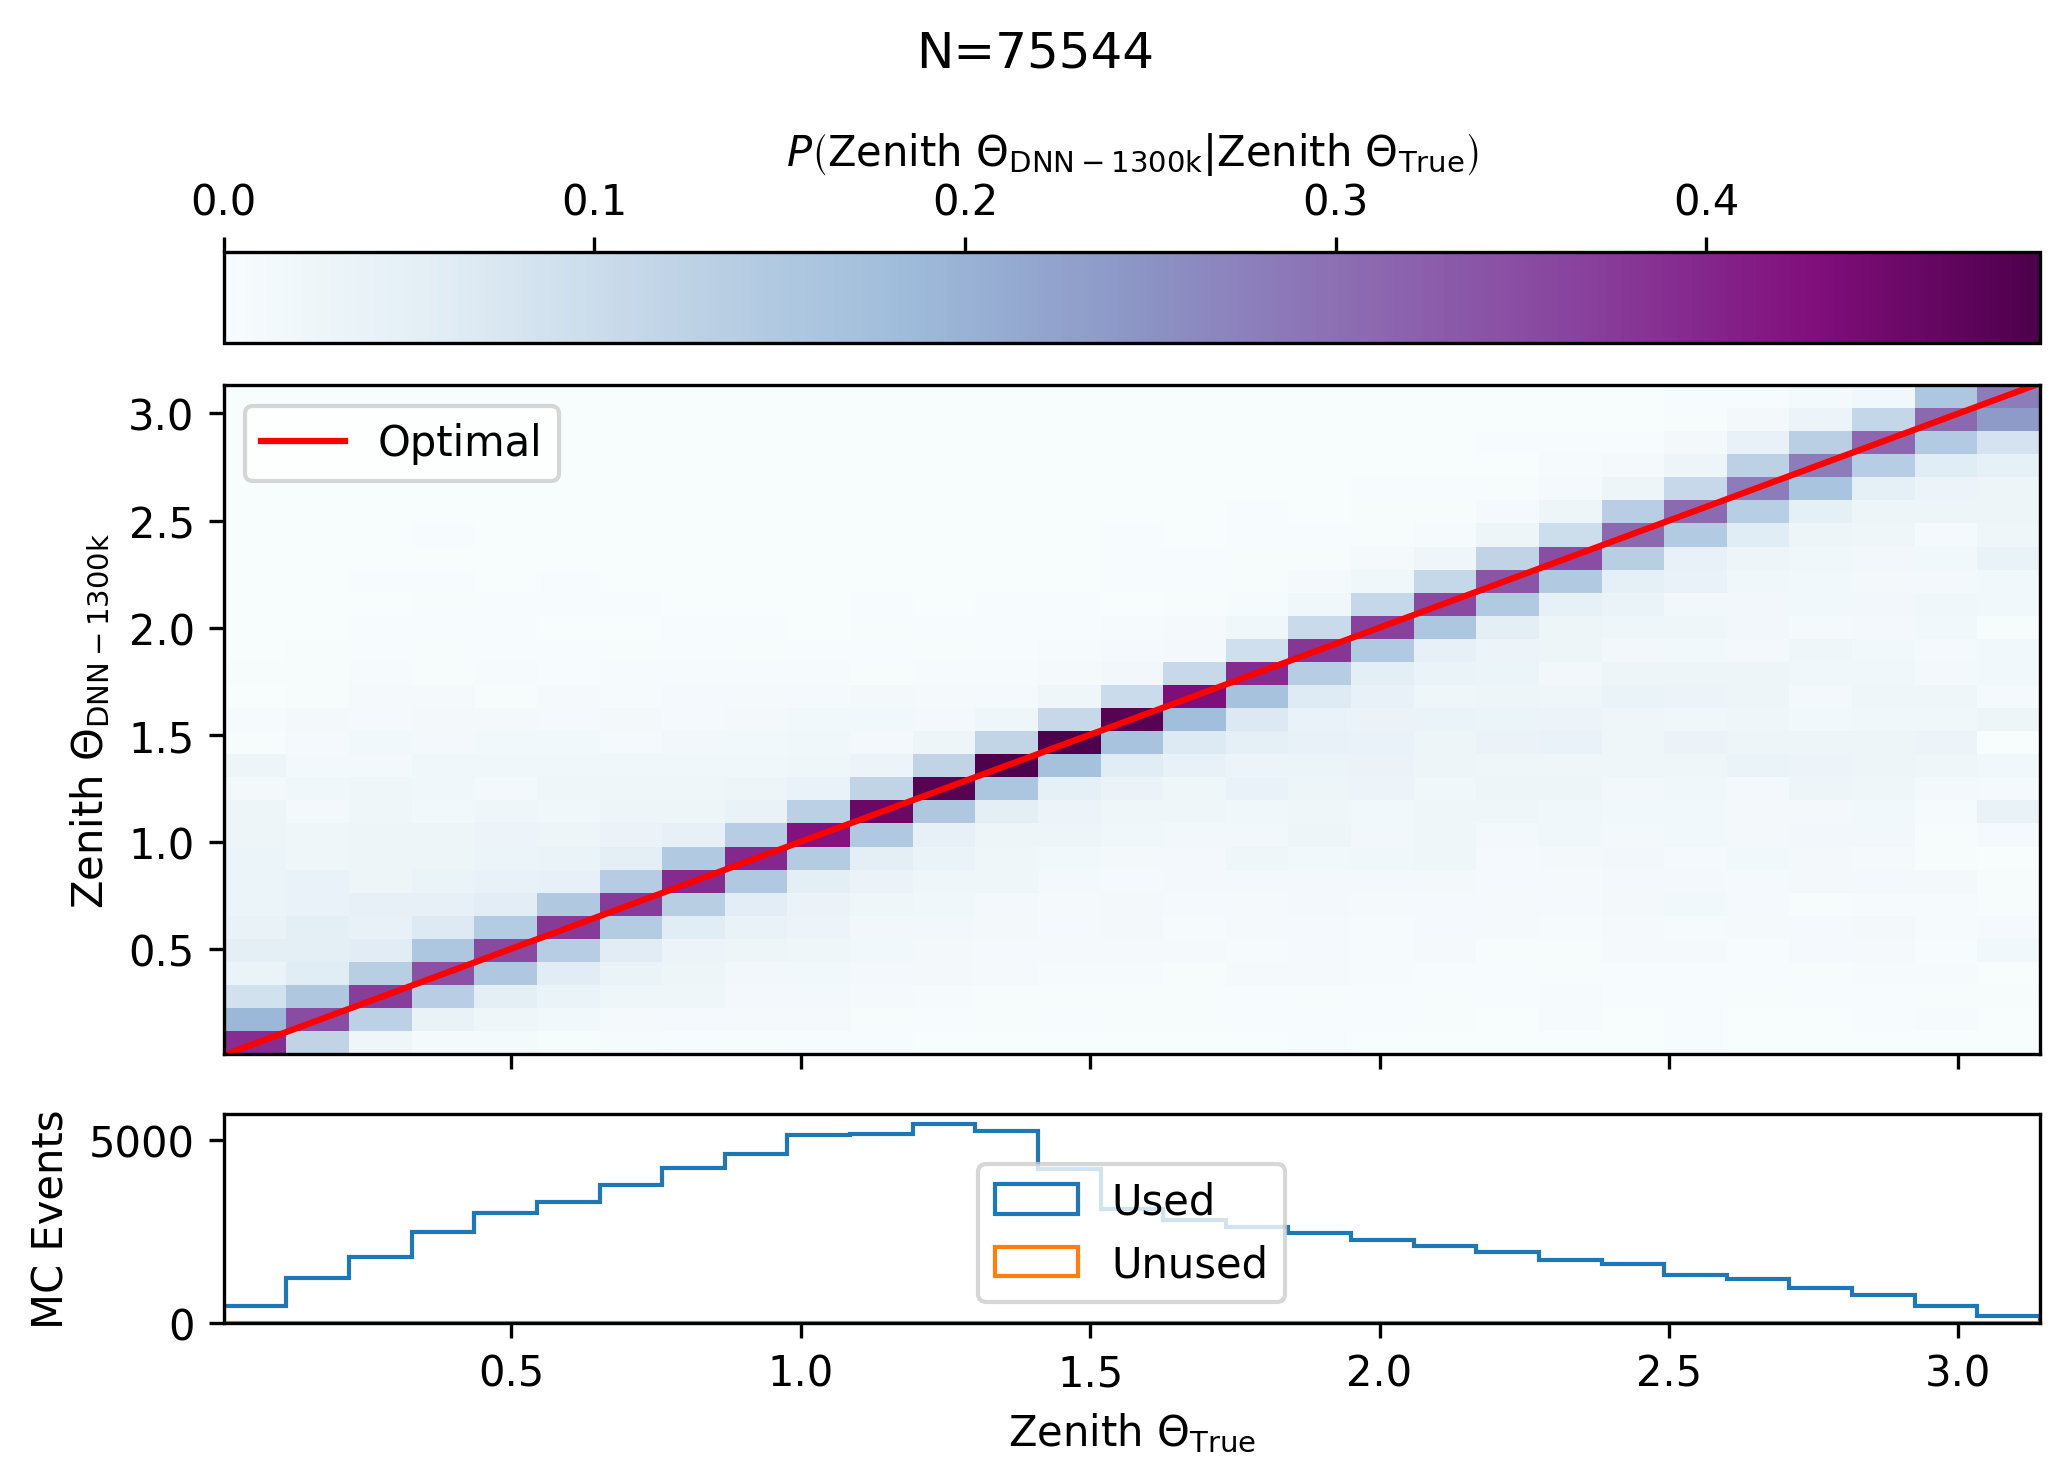
\includegraphics[width=.95\textwidth]{media/zenith_1.5m.png}
                    \caption*{\small Normalized zenith correlation @1.3m training steps}
                }
                \only<5>{
                    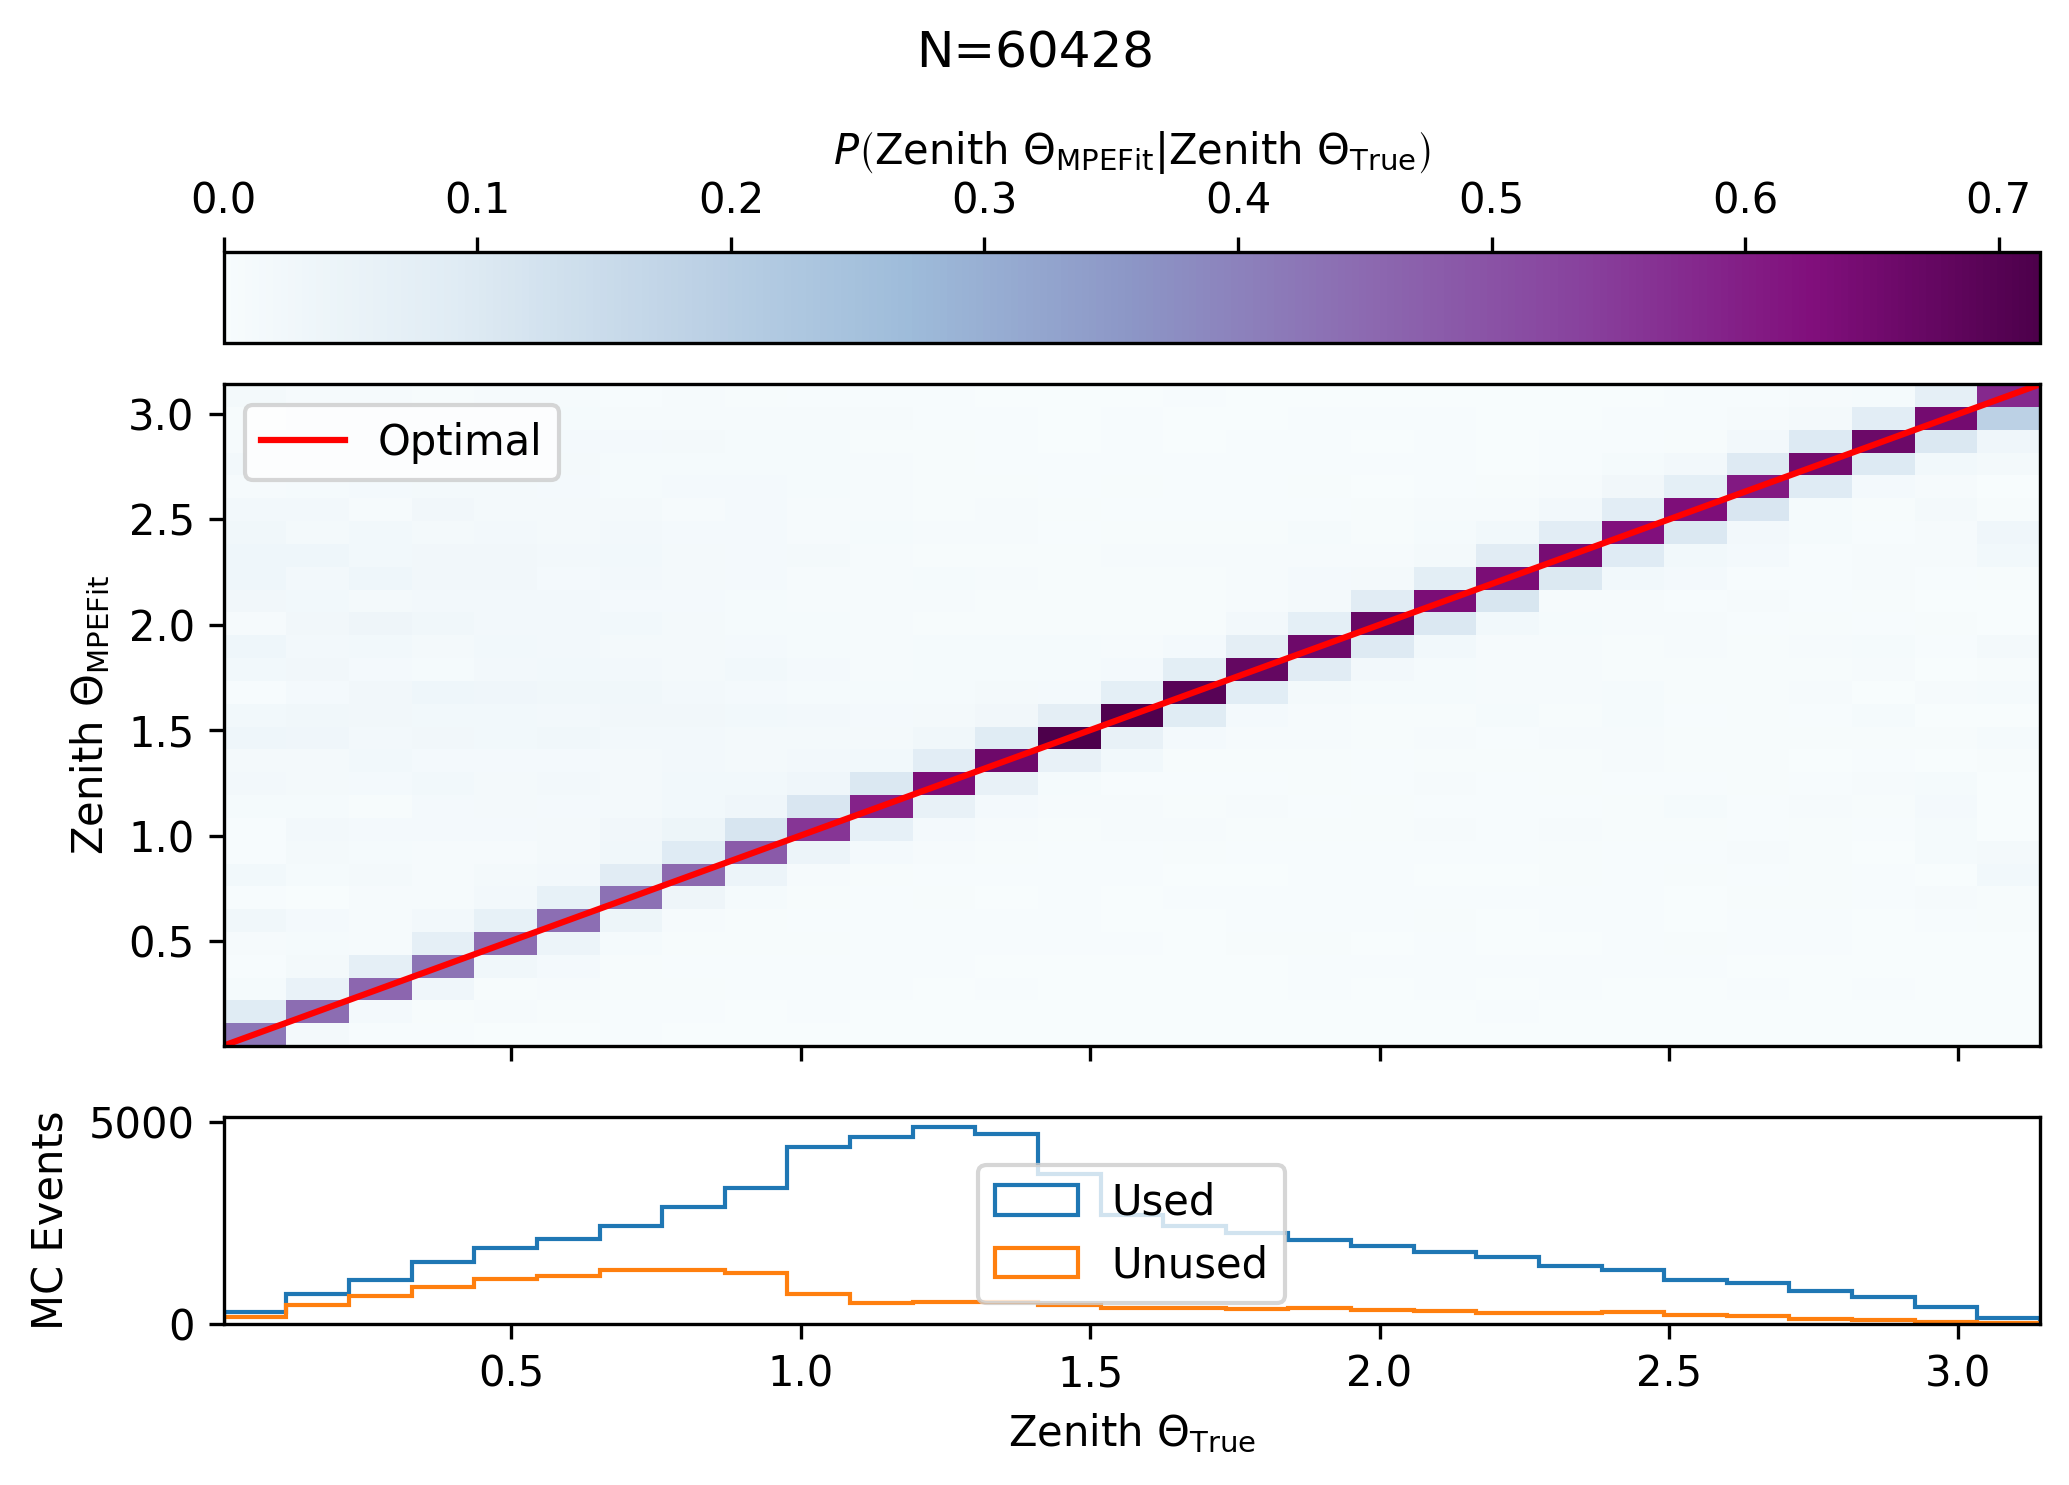
\includegraphics[width=.95\textwidth]{media/zenith_mpefit.png}
                    \caption*{\small Normalized zenith correlation for MPEFit}
                }
                \only<6>{
                    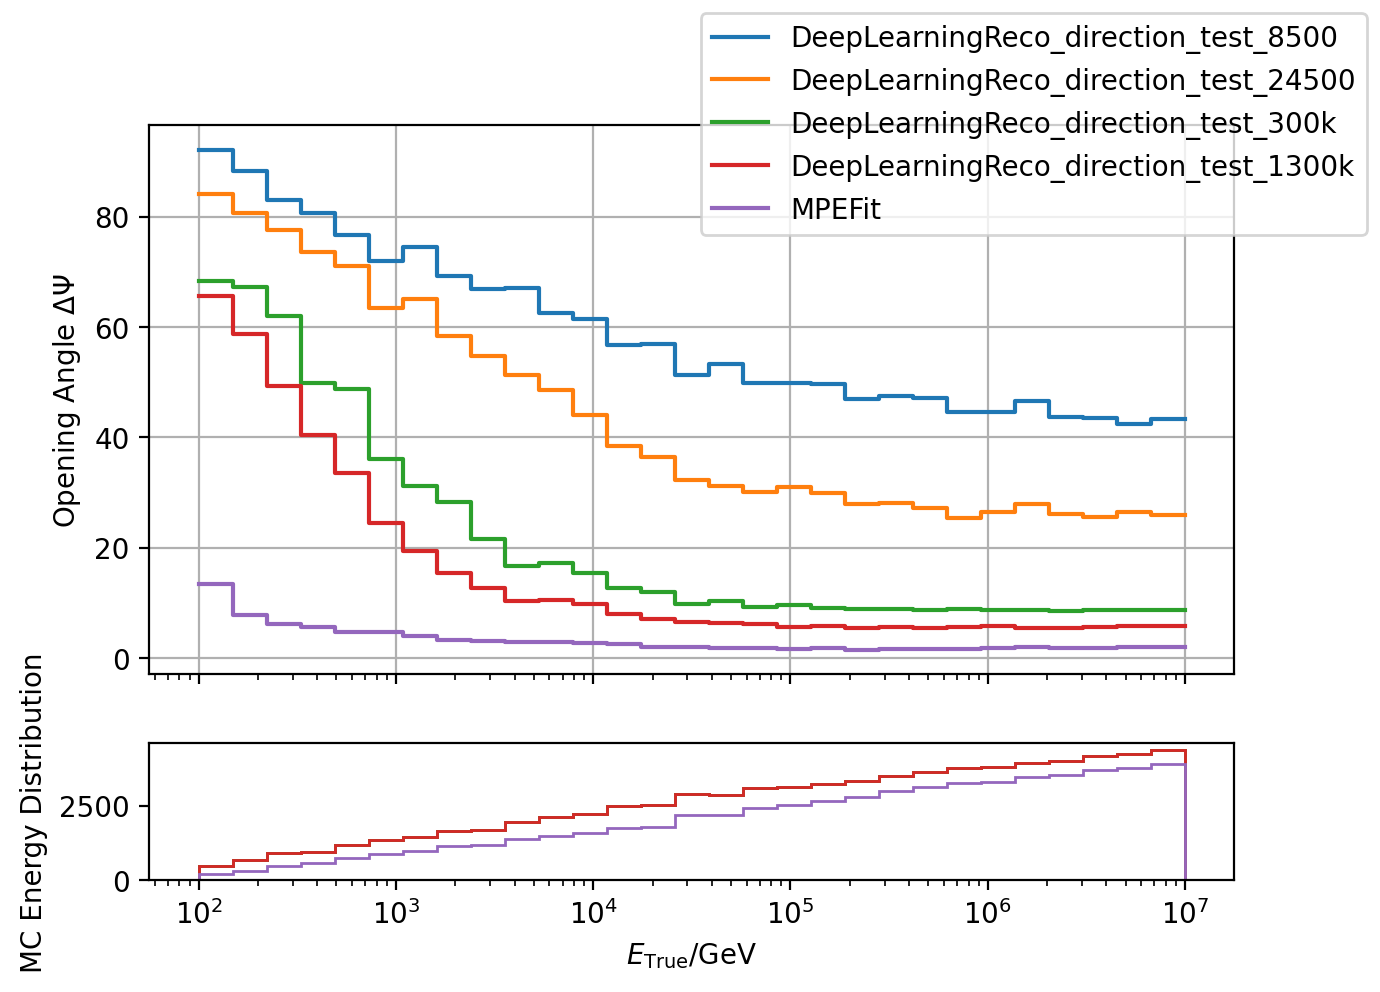
\includegraphics[width=.95\textwidth]{media/getting_started_opening_angle.png}
                    \caption*{\small Median opening angle vs. $E_\nu$}
                }
            \end{figure}
        \end{column}
    \end{columns}
\end{frame}
\begin{frame}{Generating Training Data}
    \begin{columns}
        \begin{column}{.35\textwidth}
            \begin{tabular}{>{\small\bf}r l}
                \toprule
                Features                  & 9         \\
                Training Dataset          & L2 11069  \\
                Batch Size                & 32        \\
                UDC conv. layers          & 4         \\
                LDC conv. layers          & 8         \\
                Hex. conv. layers         & 8         \\
                Dense layers              & 1\times50 \\
                $\rightarrow$ Free Params & 24532     \\
                \bottomrule
            \end{tabular}
        \end{column}
        \begin{column}{.65\textwidth}
            \begin{figure}
                \centering
                \only<1>{
                    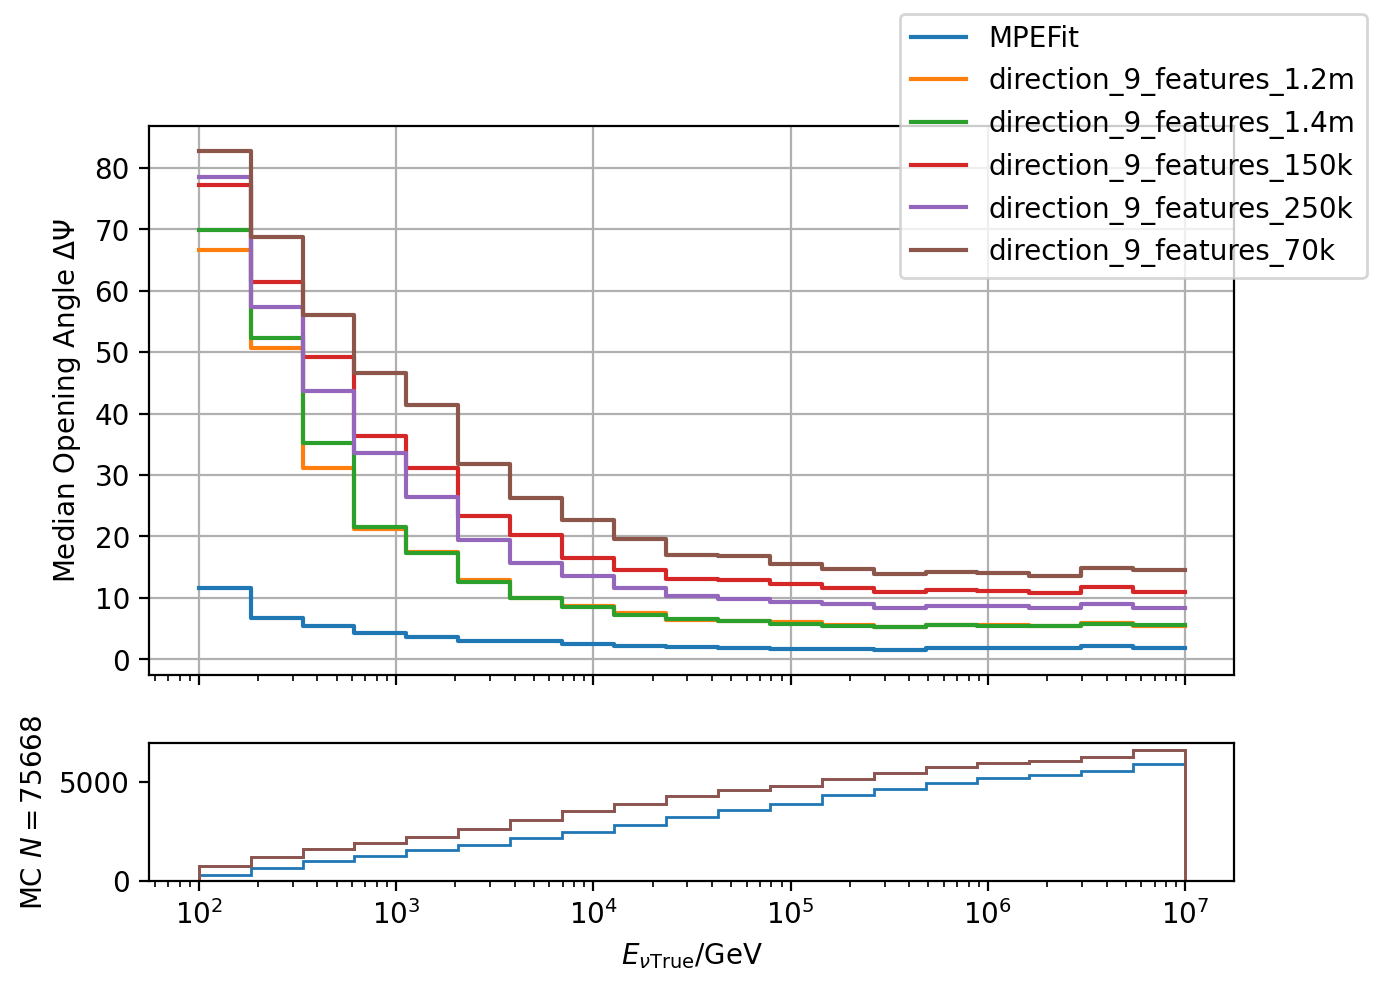
\includegraphics[width=.95\textwidth]{media/9_features_opening_angle.png}
                    \caption*{\small Median opening angle vs $E_\nu$}
                }
            \end{figure}
        \end{column}
    \end{columns}
\end{frame}
\begin{frame}{Improving the Model: Reduced Featureset}
    \begin{columns}
        \begin{column}{.35\textwidth}
            \begin{tabular}{>{\small\bf}r l}
                \toprule
                Features                  & 3         \\
                Training Dataset          & L2 11069  \\
                Batch Size                & 32        \\
                UDC conv. layers          & 4         \\
                LDC conv. layers          & 8         \\
                Hex. conv. layers         & 8         \\
                Dense layers              & 1\times50 \\
                $\rightarrow$ Free Params & 22462     \\
                \bottomrule
            \end{tabular}
        \end{column}
        \begin{column}{.65\textwidth}
            \only<1>{
                \begin{itemize}
                    \item 2070 parameters less
                    \item One test yielded 5-6 times faster training
                    \item Using
                          \begin{itemize}
                              \item total charge $c_{\mathrm{total}}$
                              \item first hit $t_{\mathrm{first}}$
                              \item charge weighted time std $t_{\mathrm{std}}$
                          \end{itemize}
                \end{itemize}
            }
            \only<2>{
                \begin{figure}
                    \centering
                    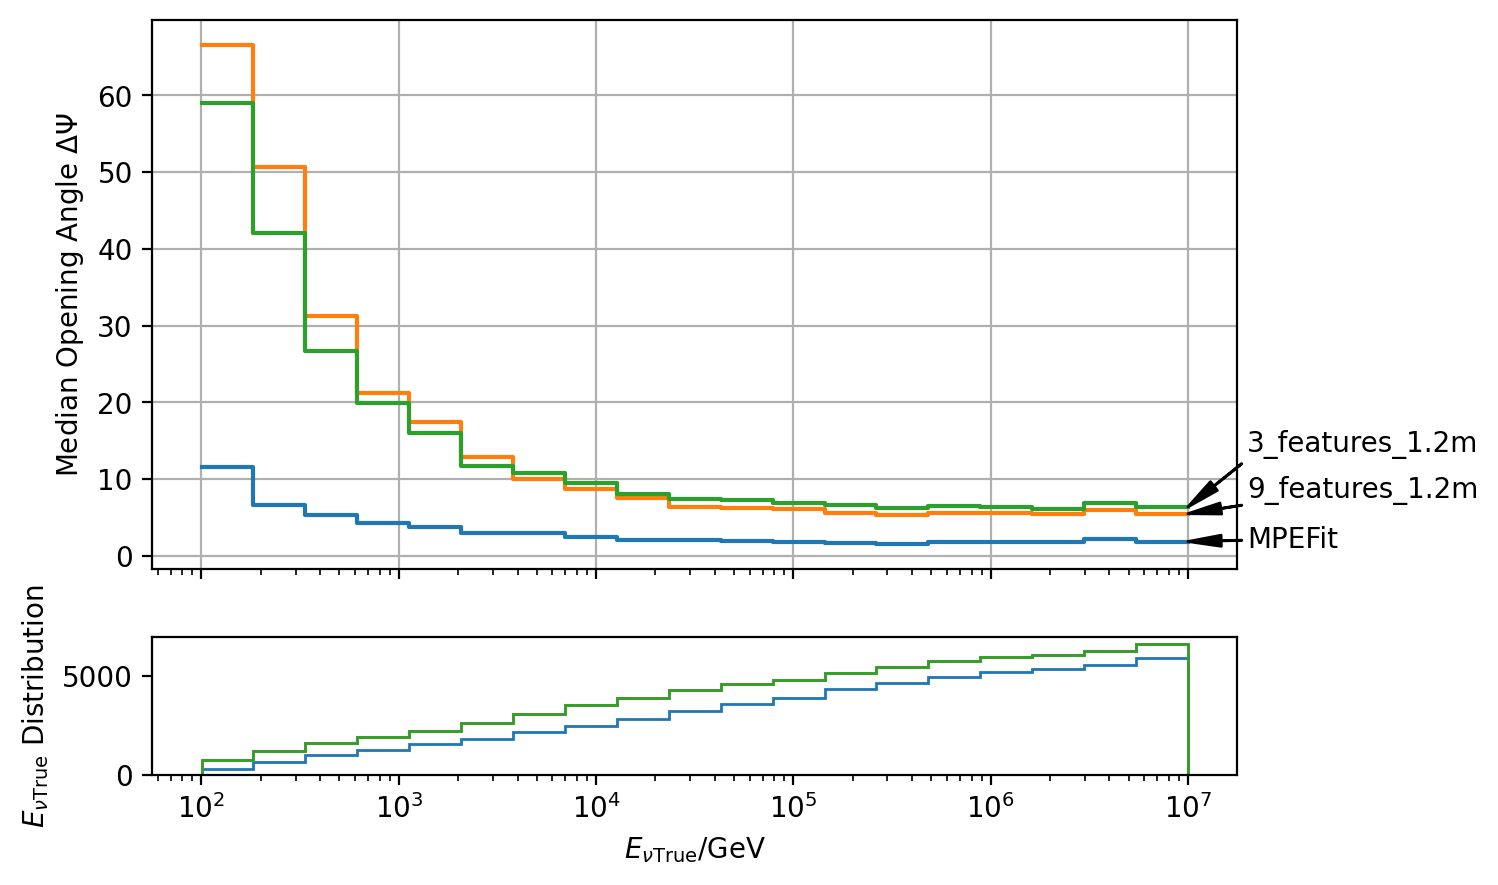
\includegraphics[width=.95\textwidth]{media/3_vs_9.png}
                    \caption*{\small Median opening angle vs $E_\nu$}
                \end{figure}}
        \end{column}
    \end{columns}
\end{frame}
\begin{frame}{Improving the Model: Higher Complexity}
    \begin{columns}
        \begin{column}{.35\textwidth}
            \begin{tabular}{>{\small\bf}r l}
                \toprule
                Features                  & 3          \\
                Training Dataset          & L2 11069   \\
                Batch Size                & 32         \\
                UDC conv. layers          & 4          \\
                LDC conv. layers          & 4          \\
                Hex. conv. layers         & 9          \\
                Dense layers              & 2\times100 \\
                $\rightarrow$ Free Params & 339467     \\
                \bottomrule
            \end{tabular}
        \end{column}
        \begin{column}{.65\textwidth}
            \only<1>{
                \begin{figure}
                    \centering
                    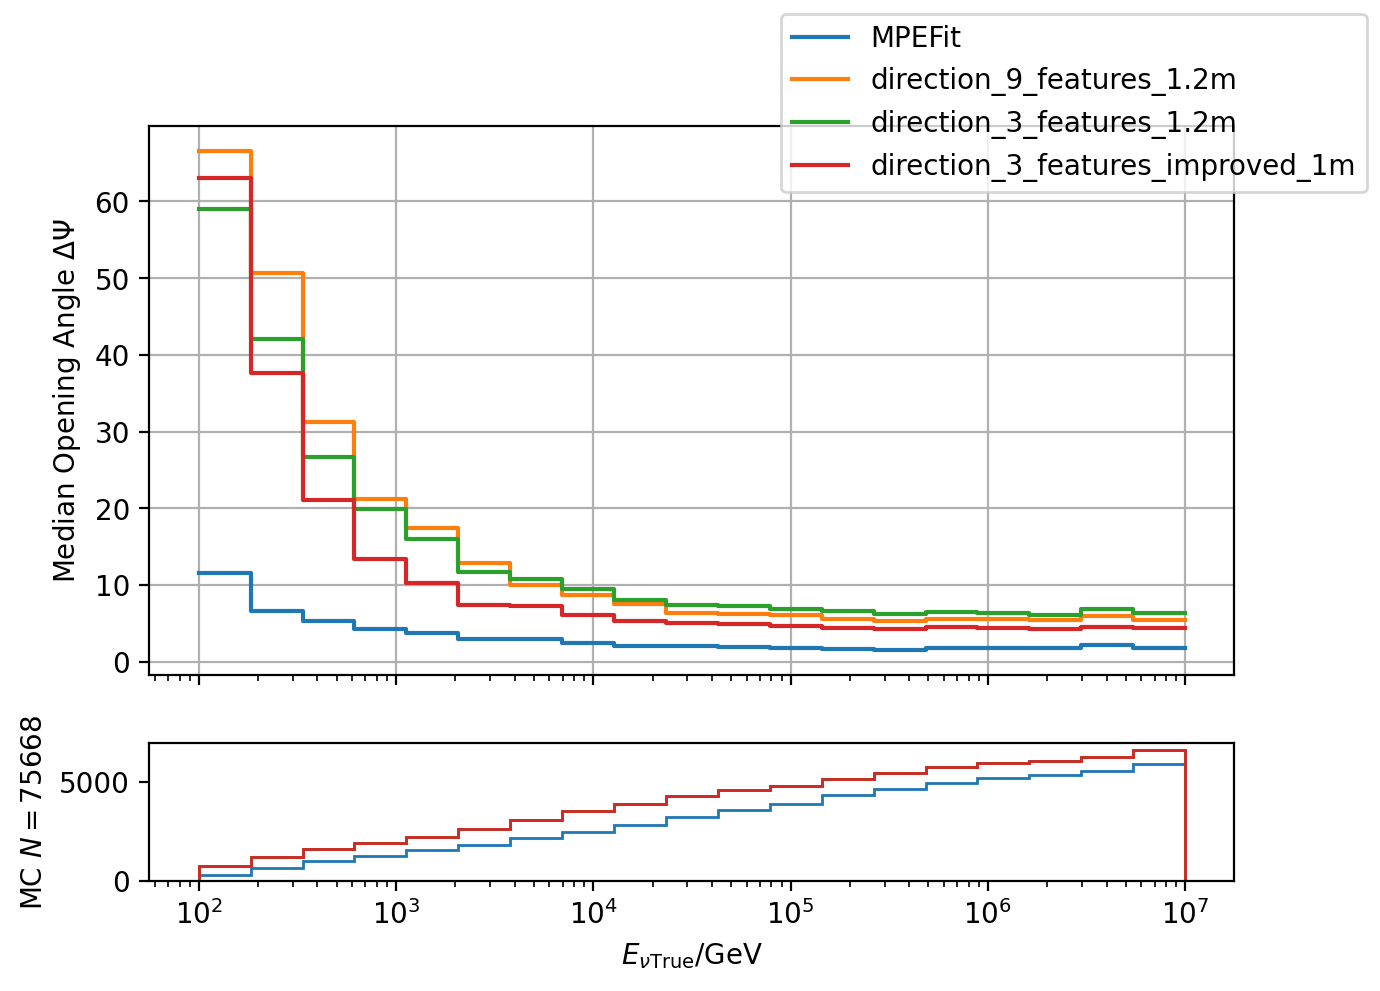
\includegraphics[width=.95\textwidth]{media/improved_model_compare.png}
                    \caption*{\small Median opening angle vs $E_\nu$}
                \end{figure}}
        \end{column}
    \end{columns}
\end{frame}
\begin{frame}{Improving the Model: Even Higher Complexity}
    \begin{columns}
        \begin{column}{.35\textwidth}
            \begin{tabular}{>{\small\bf}r l}
                \toprule
                Features                  & 3          \\
                Training Dataset          & L2 11069   \\
                Batch Size                & 32         \\
                UDC conv. layers          & 8          \\
                LDC conv. layers          & 14         \\
                Hex. conv. layers         & 20         \\
                Dense layers              & 2\times300 \\
                $\rightarrow$ Free Params & 5030912    \\
                \bottomrule
            \end{tabular}
        \end{column}
        \begin{column}{.65\textwidth}
            \only<1>{
                \begin{figure}
                    \centering
                    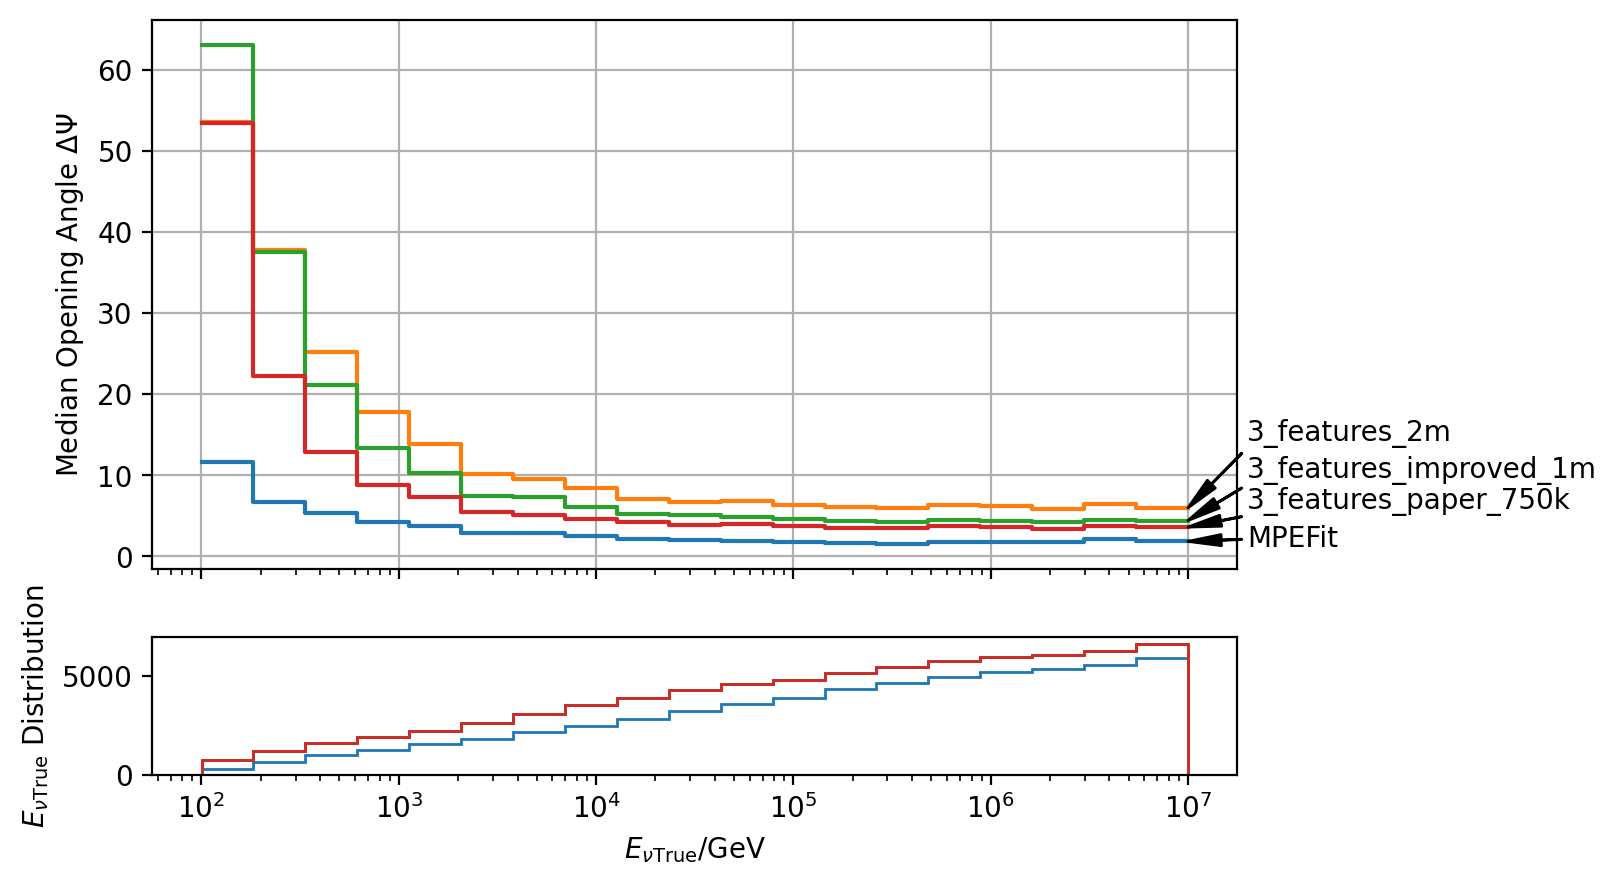
\includegraphics[width=.95\textwidth]{media/highest_complexity.png}
                    \caption*{\small Median opening angle vs $E_\nu$}
                \end{figure}}
        \end{column}
    \end{columns}
\end{frame}
\begin{frame}{Uncertainty Estimation with the High Complexity Model}
    \begin{figure}
        \centering
        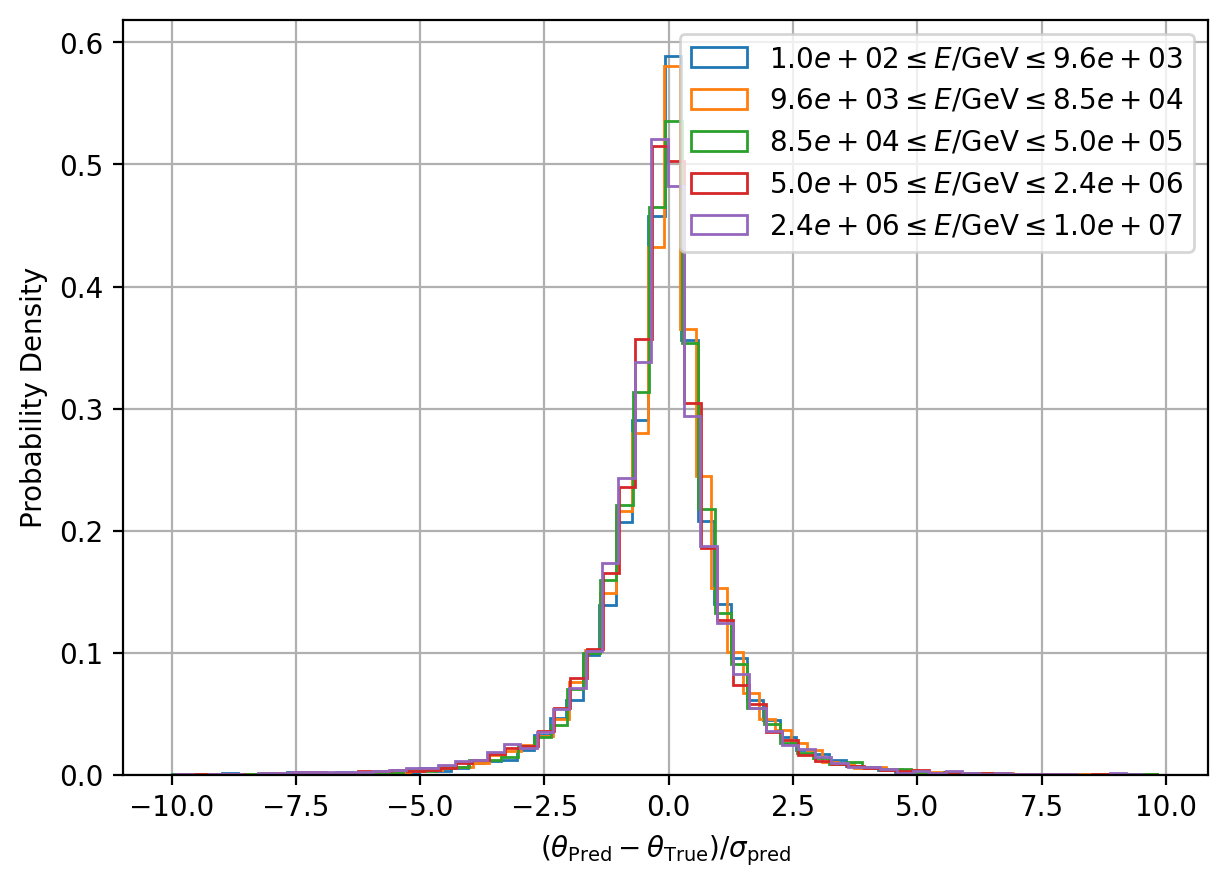
\includegraphics[width=.6\textwidth]{media/pulls.png}
        \caption*{\small Pull plot is peaked compared to expected Gaussian shape, but stable in $E_\nu$}
    \end{figure}
\end{frame}
\begin{frame}{Uncertainty Estimation with the High Complexity Model}
    \begin{figure}
        \centering
        \only<1>{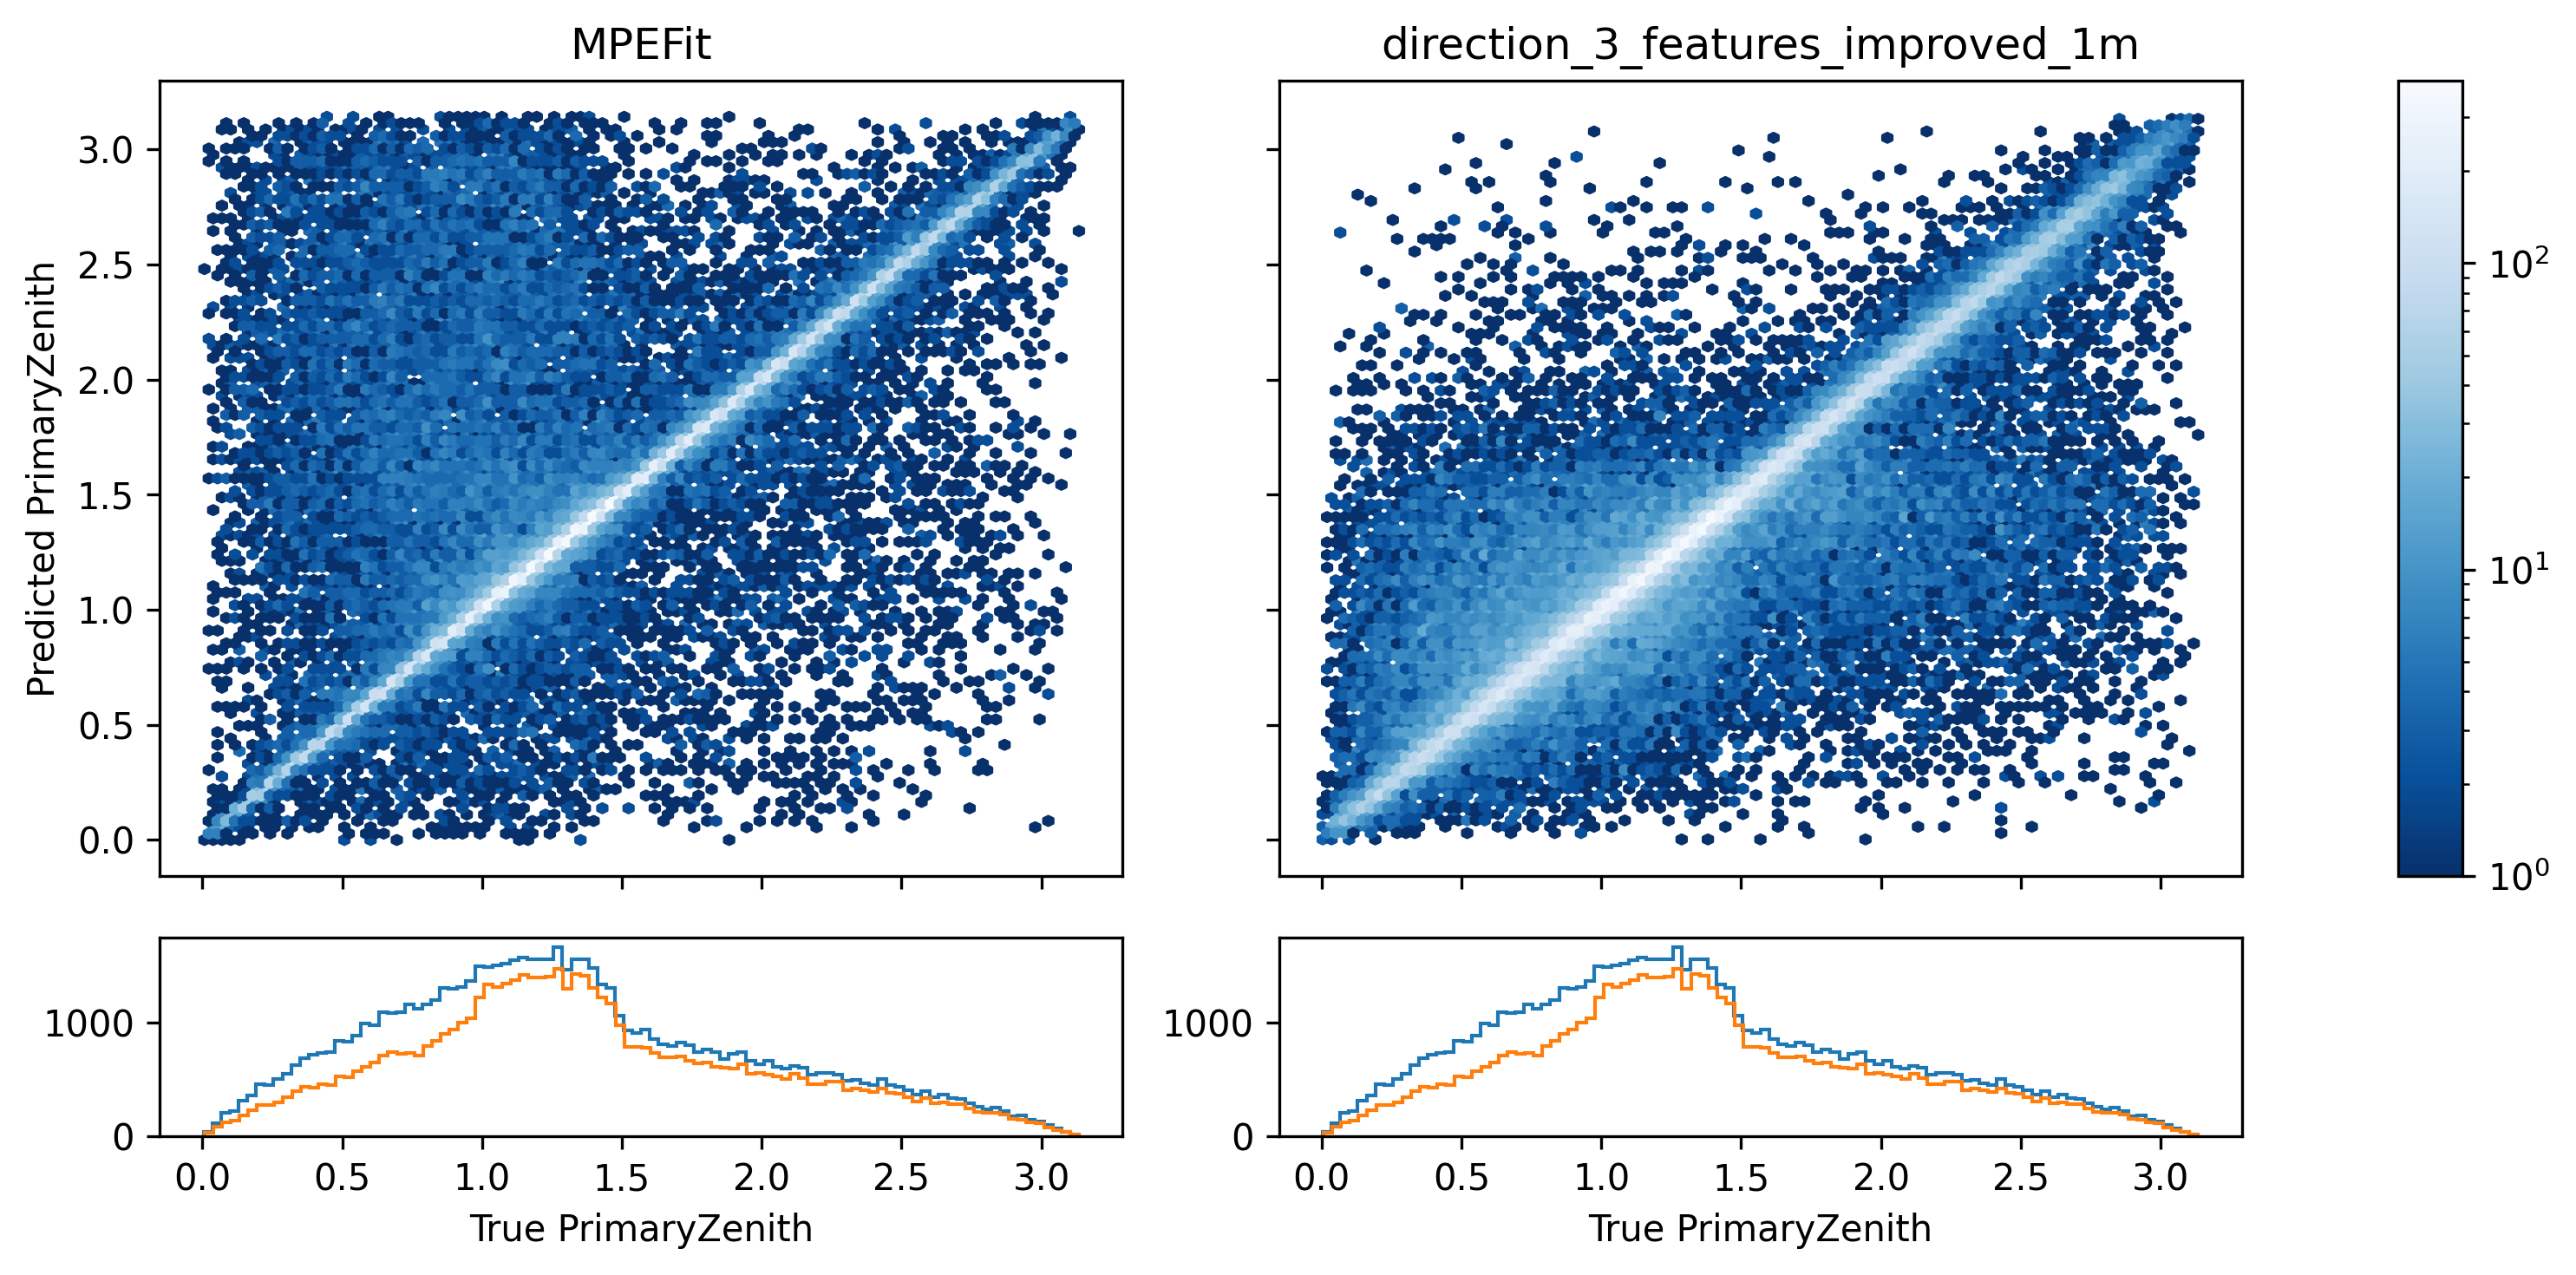
\includegraphics[width=.8\textwidth]{media/scatter_uncertainty.png}}
        \only<2>{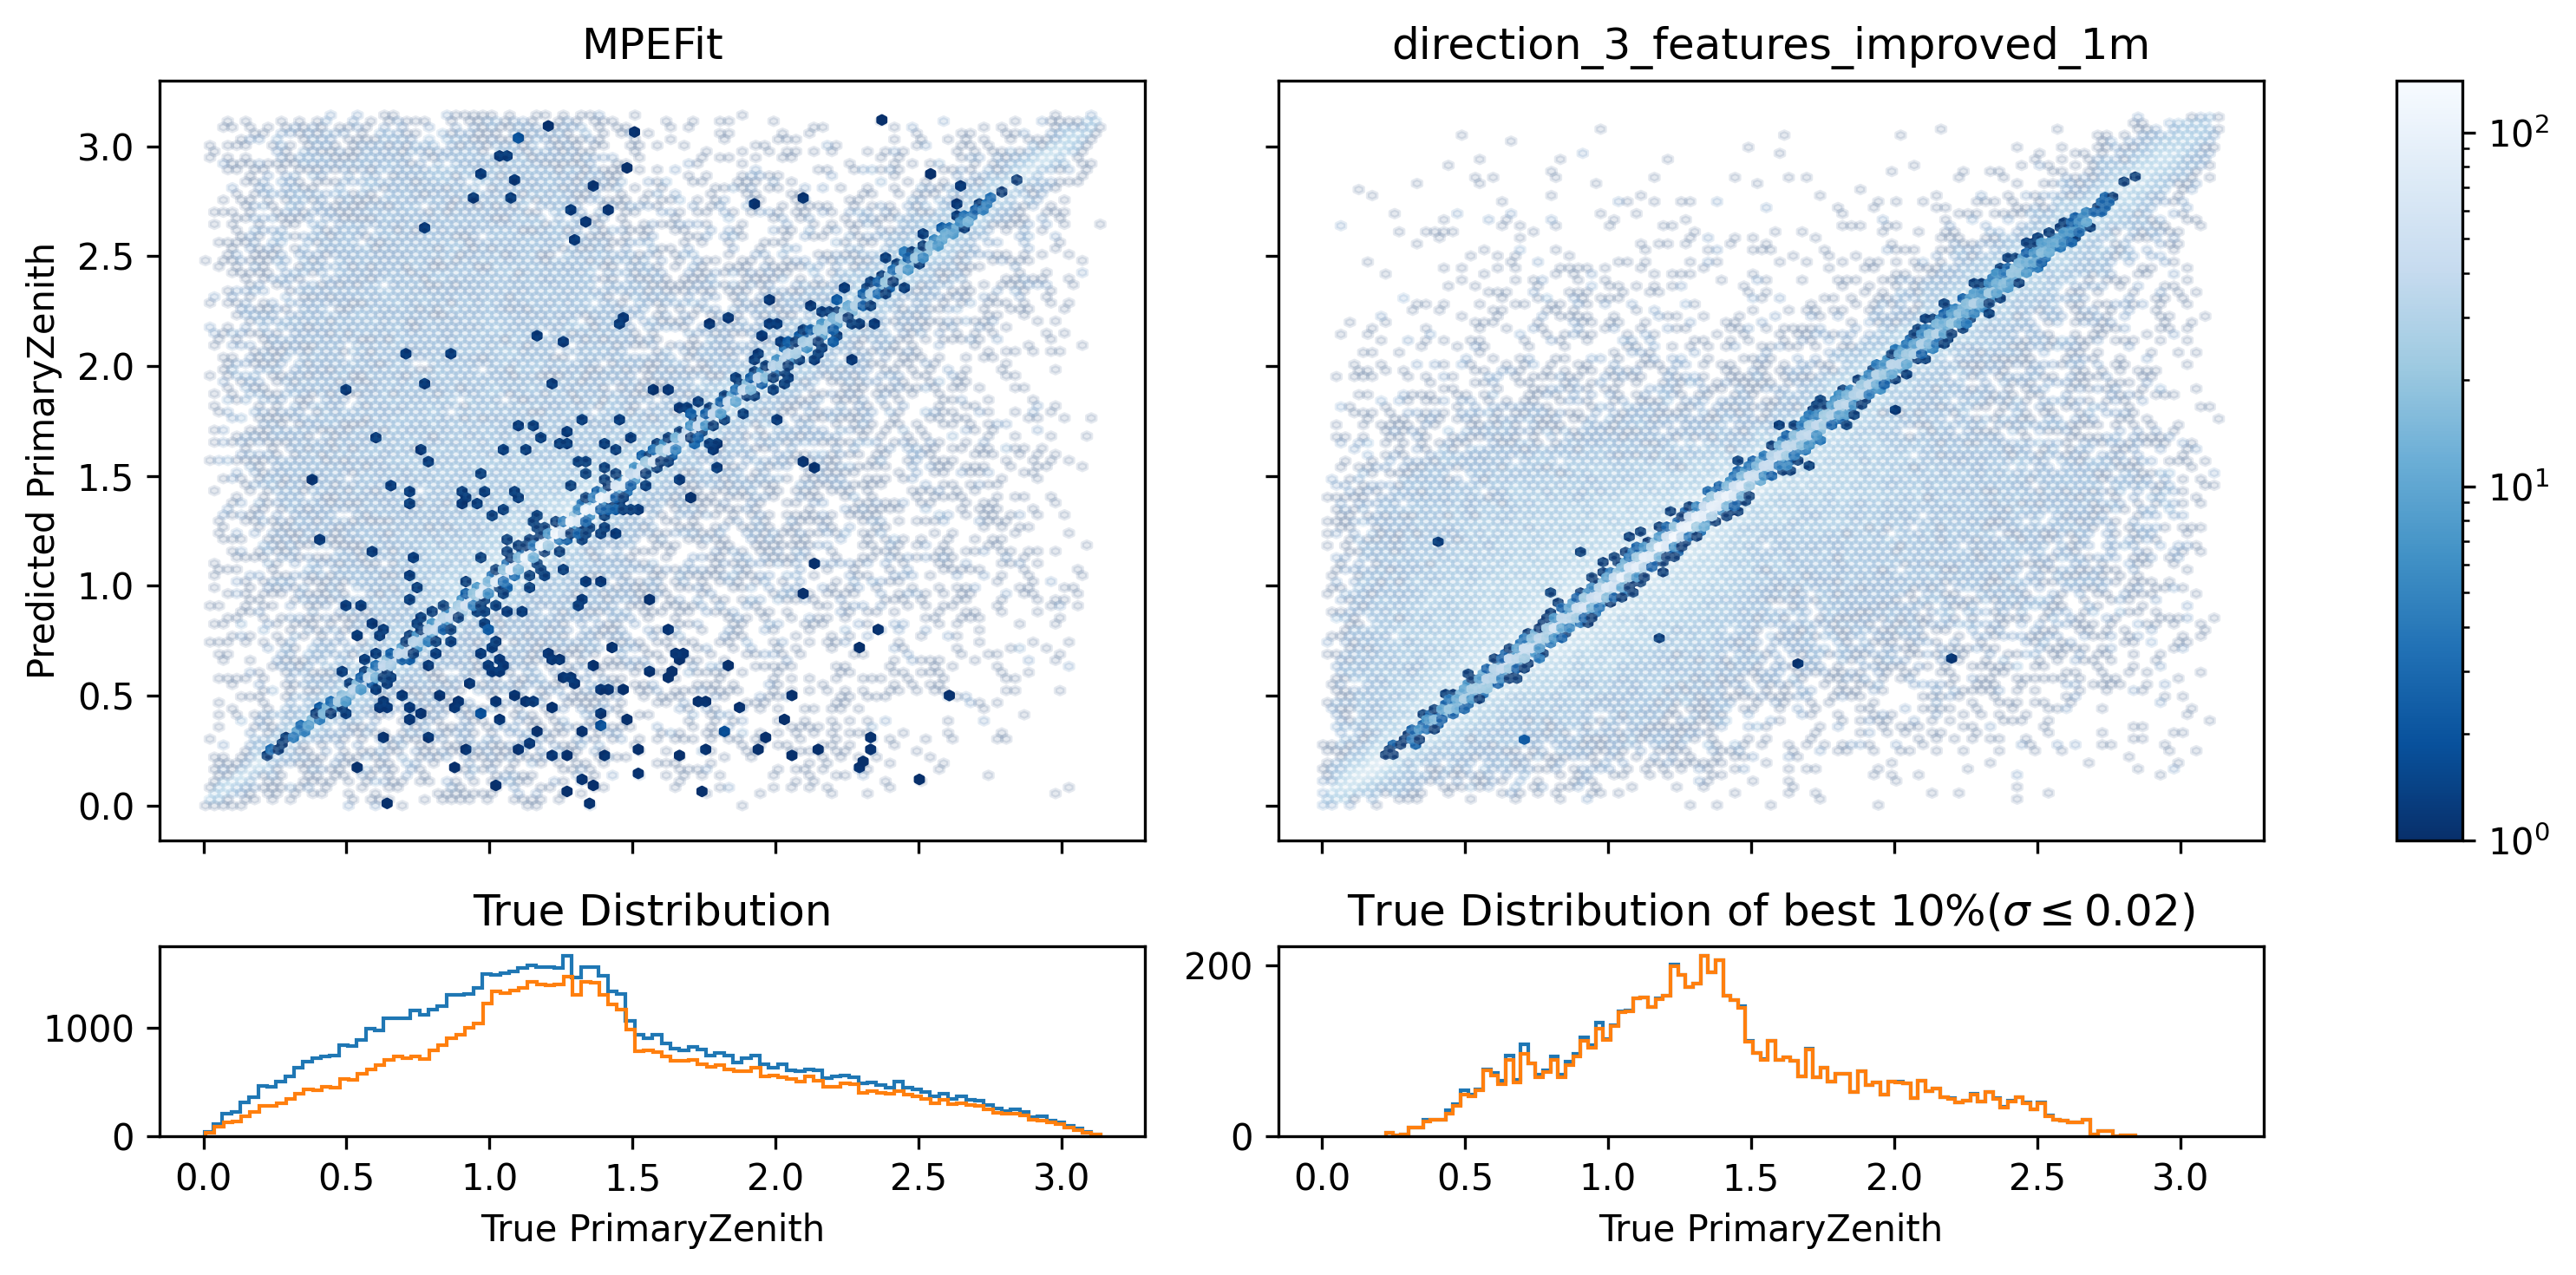
\includegraphics[width=.8\textwidth]{media/scatter_uncertainty_best.png}}
        \only<1>{\caption*{\small Hexagonal 2D-Bin plot in logarithmic color scale}}
        \only<2>{\caption*{\small Only showing 10\% of events with the lowest uncertainty estimate from DNN}}
    \end{figure}
\end{frame}